\documentclass[10pt]{article}
\usepackage[utf8]{inputenc}
\usepackage[a4paper]{geometry}
 \geometry{a4paper,total={170mm,257mm}, left=20mm, top=20mm}
\usepackage[affil-it]{authblk}
\usepackage{hyperref}
\usepackage{natbib}
\usepackage{graphicx}
\usepackage{float}
\graphicspath{ {./Images/} }

%\usepackage{multirow,booktabs,setspace,caption}
\usepackage{tikz}


\begin{document}
%\maketitle

\begin{titlepage}
\thispagestyle{empty}
\begin{center}%
  	{\LARGE Master Thesis \par}
  	\vskip 3em
  	{\line(1,0){100} \par}
  	\vskip 0.75em
    {\LARGE \textbf{Empirical validation of the contrast avoidance model using social media sentiment analysis} \par}%
    \vskip 3em%
    {\large
      \begin{tabular}[t]{c}%
        Alex Hartmann
      \end{tabular}\par}%
     \vskip 0.75em
		{\line(1,0){100} \par}
      \vskip 10em%  
    {\small Thesis submitted in partial fulfillment \\
    of the requirements for the degree of \\ Master of Science
    of Data Science for Decision Making \\ at the Department of Advanced Computing Sciences\\
		of the Maastricht University \par}%
      \vskip 3em%
    {\normalsize \textbf{Thesis Committee:}\\
	    \vskip .5em% 
	    \begin{tabular}[t]{c}%
	       Dr. Marijn ten Thij\\Christof Seiler
      \end{tabular}\par}%	
    	\vfill
    {\small \begin{center} 
      Maastricht University\\
      Faculty of Science and Engineering\\
      Department of Advanced Computing Sciences %\\
%      Master \@department
    \end{center} \par}%
    \vskip 2.5em%
    {\normalsize \today \par}%       % Set date in \large size.
  \end{center}
\end{titlepage}

\setcounter{page}{1}

%summary of whole research. Include:

% Objective
% Methods
% A rough description of outcome


\section*{Abstract}

The contrast avoidance model (CAM) posits that anxiety patients attempt to avoid large shifts in emotional states and therefore maintain a heightened state of negative affect (NA). Previous research showed that this can be empirically supported using VADER sentiment estimations of Twitter data and aggregating the sentiment scores for each user, comparing an anxiety cohort with a depression cohort. In order to build upon that, the present study constructed new aggregation mechanisms. To give less weight to short-term fluctuations in NA levels, tweets are aggregated in a 6-hour rolling window and a daily window for each user separately. Then, the cohorts are compared with regards to their NA levels and variability. It was found, that depression patients show higher NA levels as well as variability when examining VADER scores. A novel analysis method based on linear mixed modeling (LMM) was proposed. LMMs were fit to the different aggregation levels and the estimated regression coefficient for the anxiety cohort was used as a measure of differences in general NA levels, while the residual standard deviation was used as a measure of unpredictability and thus NA variability that cannot be explained by available external factors. The analysis showed that this approach also supports the previous findings when applied to VADER sentiment scores, indicating that depression patients have higher NA levels and higher NA variability. When applying the proposed methods to sentiment scores obtained from transformer-based NLP tools (specifically, a RoBERTa model), the results changed. NA levels were still significantly higher for depression patients, but no differences or even opposite significant differences in NA variability were found. In the LMM approach with 6-hour windowed data, the anxiety cohort showed significantly larger NA variability than the depression cohort. Thus, the previous findings regarding empirical validation of the CAM could only be supported for VADER-based analysis and require future research in order to explain the conflicting results.




%------------------------------------------------
%	Sections
%------------------------------------------------

%\begin{multicols}{2}

\section{Introduction}
\label{sec:intro}


Anxiety and depression are among the most widespread mental health disorders, significantly affecting global public health. According to the World Health Organization (WHO), depression is one of the worldwide leading causes of disability, with over 280 million people affected by it \citep{who2023depression}, while anxiety disorders are the most prevalent mental disorders in the world, impacting over 300 million individuals annually~\citep{who2023anxiety}. These disorders not only reduce individual quality of life but also impose substantial economic burdens on public healthcare systems.

Anxiety and depression have distinct diagnostic criteria. Since they frequently co-occur, thier clinical assessment and treatment can be quite complicated though~\citep{kessler2003epidemiology}. Anxiety is typically characterized by excessive worry and heightened physiological arousal, whereas depression involves feelings of persistent sadness, loss of interest, and cognitive symptoms~\citep{apa2013dsm}. However, shared mechanisms, such as heightened emotional dysregulation and stress susceptibility, suggest an overlapping origin.

One framework that offers insight into anxiety's persistence and overlap with depressive symptoms is the Contrast Avoidance Model (CAM). The CAM posits that individuals with anxiety disorders are motivated to maintain a state of heightened negative affect to avoid sharp emotional shifts when confronted emotionally taxing situations~\citep{newman2011contrast}. This sustained negativity may serve as a maladaptive strategy for reducing unpredictability in emotional experiences but can also perpetuate chronic stress and predispose individuals to depression~\citep{llera2014emotional}.

Empirically validating the CAM is essential to advancing our understanding of anxiety and its relationship with depression. By establishing robust evidence for the mechanisms proposed by the CAM, researchers can better differentiate it from other theoretical frameworks and identify specific pathways for intervention. For instance, interventions targeting the cognitive and emotional strategies associated with contrast avoidance may help disrupt the cycle of sustained worry and emotional distress. Furthermore, empirical support for the CAM could inform personalized treatment approaches, optimizing therapeutic outcomes for individuals with anxiety and co-occurring depressive symptoms.

Attempts at validating the CAM have been made before. For example, \citet{cam_questionnaire} developed a questionnaire that empirically shows the workings of the CAM. Further, \citet{rutter2024} use public Twitter data to investigate differences in negative affect variability and levels between anxiety and depression patients. One advantage of their approach over the questionnaire is that they did not use self-reported data (i.e., responses to a survey) but rather sentiment analysis as a measure of negative affect on public Tweets. 

\citeauthor{rutter2024} found that the anxiety cohort did show lower levels of negative affect variability than the depression cohort, which is in keeping with the CAM. They used tweets data for individuals and applied the Valence Aware Dictionary for sEntiment Reasoning (VADER) \citep{vader} to obtain negative affect scores for each tweet. Then, they grouped the individuals into an anxiety and a depression cohort depending on the availability of a tweet indicating clinical diagnosis of either. They computed an overall mean negative affect level and a negative affect standard deviation for each individual and compared the distributions grouped by cohort membership.

Although their research provided valuable insights into empirical assessment of the CAM, their methods exhibit several weaknesses. First, VADER as a rule- and dictionary-based sentiment analyzer is a relatively simple sentiment analysis tool that does not consider the broader context of the text in which it was written. While VADER does handle tasks like negation to a certain degree, it can often fail with more complex sentences and sarcasm \citep{understandingVADER}. This could prove to be a significant weakness to the methodology.

Second, \citeauthor{rutter2024} computed negative affect levels and variability as a mean and standard deviation across the entire time series for each individual. Thus, they fail to capture short-term fluctuations in negative affect levels.

Third, and possibly most importantly, they did not control for external influential factors that determine negative affect levels. For example, \citet{bathina2021Covid} showed that negative affect levels and overall well-being are heavily influenced by global events such as the COVID-19 pandemic and the \textit{Black Lives Matter} riots in the United States. Further, \citet{tenthij2020circadian} found evidence that negative affect levels as displayed by online activity depend on the time of day. In particular, online activity is related to the circadian rhythm of individuals. \citet{dzogang2017seasonal} showed how mood levels depend on the seasons, with \citet{denissen2008weather} further underlining this by showing how mood depends on weather, which in turn is related to seasonality. These are just a few of the studied predictors of mood levels, which were all disregarded by the previous study. 

Additionally, this study aims to address the limitations of prior research by implementing methodological improvements that offer a more nuanced analysis of negative affect variability in individuals with anxiety and depression. By applying moving window aggregations, we aim to capture short-term fluctuations in emotional states rather than relying solely on static measures like mean and standard deviation over an extended period. Moving window aggregations are powerful tools for extracting localized patterns and trends within sequential data. By summarizing a fixed-length segment of data at each step—typically using functions such as mean, median, or variance—this technique enables researchers to observe how a system's behavior evolves over time without losing resolution across the full dataset. This dynamic approach enables a more precise assessment of affective instability, a key characteristic of both anxiety and depression.  

Furthermore, by incorporating linear mixed-effects models, we seek to account for individual-level variability and control for external influences that may confound the relationship between affect variability and diagnostic group membership. Unlike simple mean comparisons, mixed-effects models allow us to analyze the impact of contextual factors such as time of day, seasonal trends, and major global events on negative affect levels. This approach enhances the robustness of our findings by isolating the unique contribution of contrast avoidance to affective patterns in anxiety and depression.  

Ultimately, this study aims to refine our understanding of the Contrast Avoidance Model and its empirical validity. By addressing key methodological concerns and leveraging improved analytical techniques, we strive to provide more reliable insights into the emotional dynamics of anxiety and depression. These findings have the potential to inform clinical interventions by identifying more precise targets for therapy and improving the personalization of treatment strategies for individuals struggling with anxiety-related and depressive symptoms.

Therefore, the goal of this article is to build upon the findings of \citeauthor{rutter2024} and further test their validity. This is done by investigating two research questions. 

\begin{itemize}
    \item Can the findings of \citeauthor{rutter2024} be replicated by using moving window aggregations of negative affect levels?
    \item Can the findings of \citeauthor{rutter2024} be replicated by using linear mixed effects models to build a predictive model of negative affect levels and investigating the unexplained variance?
\end{itemize}






%\input{Sections/2_RelatedWorks}

\section{Data}
\label{sec:data}

Between January 1st 2018 and January 1st 2019 samples of daily tweets were searched using the Observatory on Social Media (OSoMe; 48). OSoMe of the Indiana University Network Science Institute (IUNI) provides access to 10\% of tweets each day. To construct the cohorts OSoMe was searched using the query „diagnos*” as well as different specific internalizing disorder queries (e.g., „anxiety”, „OCD”, „depression”).  Based on the previously described inclusion approach (44, 49), social media users were gathered who have stated to have an actual clinical diagnosis of either anxiety or depression. An example statement would be „my doctor diagnosed me with depression”. Self diagnoses, such as „I must be depressed”, were excluded. Afterwards the gathered tweets were searched for the words „i”, „diagnos*”, „depres*/ anx*” in that order in a case-insensitive manner. to match the greatest variety of diagnosis statements. The queries were then combined to obtain the greatest variety of self-referential diagnosis statements within the tweets. 

The subjects were then grouped into an anxiety (A) cohort and a depression (D) cohort based on these statements about clinical diagnoses. All people who exhibited diagnoses for both anxiety and depression were excluded from the analyses.

Based on the results of a comparative analysis of social media sampling methods by Ernala et al (2019; „Methodological Gaps in Predicting Mental Health States from Social Media: Triangulating Diagnostic Signals.”) it was ensured that only self-referential tweets of a clinical diagnosis of either depression or anxiety were included. Thus, the remaining statements were assessed using three judges. They decided whether a tweet was self-referential and excluded perceived jokes, quotes or external references. Only statements that were unanimously rated as self-referential of a clinical diagnosis were kept in the dataset. As Chancellor and Choudhury (2019; „Methods in predictive techniques for mental health status on social media”) propose, conclusions in regards to depression’s population morbidity and its language features based on the use of data-driven supervised machine learning approaches were avoided. 

Using the Twitter „user\_timeline” API endpoint (https://developer.twitter.com/en/docs/tweets/timelines/api-reference/get-statuses-user\_timeline) the timeline for each Twitter user who has made a qualifying statement was gathered. All retweets and all tweets in a different language (i.e. non-English) were removed. Further, tweets posted before January 1st 2018 were excluded as they predate the diagnosis reference that was referred to. 

Lastly, to ensure that only accounts belonging to individuals were included, M3 and Botometer were used. M3 is a demographic classification algorithm assessing accounts to be an organization or institution. Similarly Botometer is a software identifying automated accounts (bots).

Some demographic information, while not usually publicly available for social media profiles, was estimated. Machine learning methods exist for estimating demographics from profiles online. For example, for this article, \textit{M3} \citep{m3} was used to predict a user's age and gender. It predicts a gender propensity for each user. If the probability of gender classification is greater than $80\%$, an individual is labeled as either male or female (Macro-F1: $0.915$). Age was classified into the cateogories “18 and below”, “19–29”, “30–39”, and “40 and up”. The model achieves a Macro-F1 of $0.425$ for age categorization.

\subsection{Inferring time zone information}

User activity on social media platforms such as Twitter is strongly influenced by the time of day. For instance, individuals tend to be significantly less active during nighttime hours when they are likely to be asleep, and more active during waking hours, typically corresponding to their local daytime. In datasets comprising globally distributed users, this diurnal variation necessitates accounting for users' time zones when analyzing temporal patterns of activity or sentiment. Failing to do so can obscure meaningful trends or introduce systematic biases into the analysis.

However, explicit time zone information is available for only a small fraction of users—specifically, 419 users in this dataset who have provided self-reported location data that could be reliably mapped to a time zone. To enable time-of-day-based analyses at scale, it becomes essential to infer the time zones of the remaining users. To address this, an inference algorithm was developed that leverages the temporal distribution of each user’s tweeting activity. By analyzing frequency distributions across UTC-based timestamps, the algorithm aims to estimate the most probable time zone for each user.

First, the 419 users with known time zones were used to construct a reference distribution of tweet activity. This distribution represents the proportion of tweets posted at each hour of the day, rounded to the nearest full hour. It served as a baseline pattern for identifying the most likely local time of activity.

For users without known time zones, their timestamps were systematically adjusted across all possible UTC offsets from -12 to +15 hours. For each possible offset, a new hourly distribution of tweet activity was computed. We selected the best offset by minimizing the mean absolute error (MAE) between the shifted distribution and the reference distribution.

To evaluate the effectiveness of this approach, the 419 users with known time zones were used as a test set, meaning their actual time zones were compared with the inferred ones. However, this introduced a degree of bias, as the reference distribution was derived from the same users being evaluated.

The results indicated that the algorithm exactly matched the correct time zone in only 19.33\% (0.1933) of cases. However, the accuracy improved when considering slight deviations: in 57.76\% (0.5776) of cases, the predicted time zone was within one hour of the correct value. The accuracy depending on tolerance level is visualized in Figure \ref{fig:time-zones}.

\begin{figure}
    \centering
    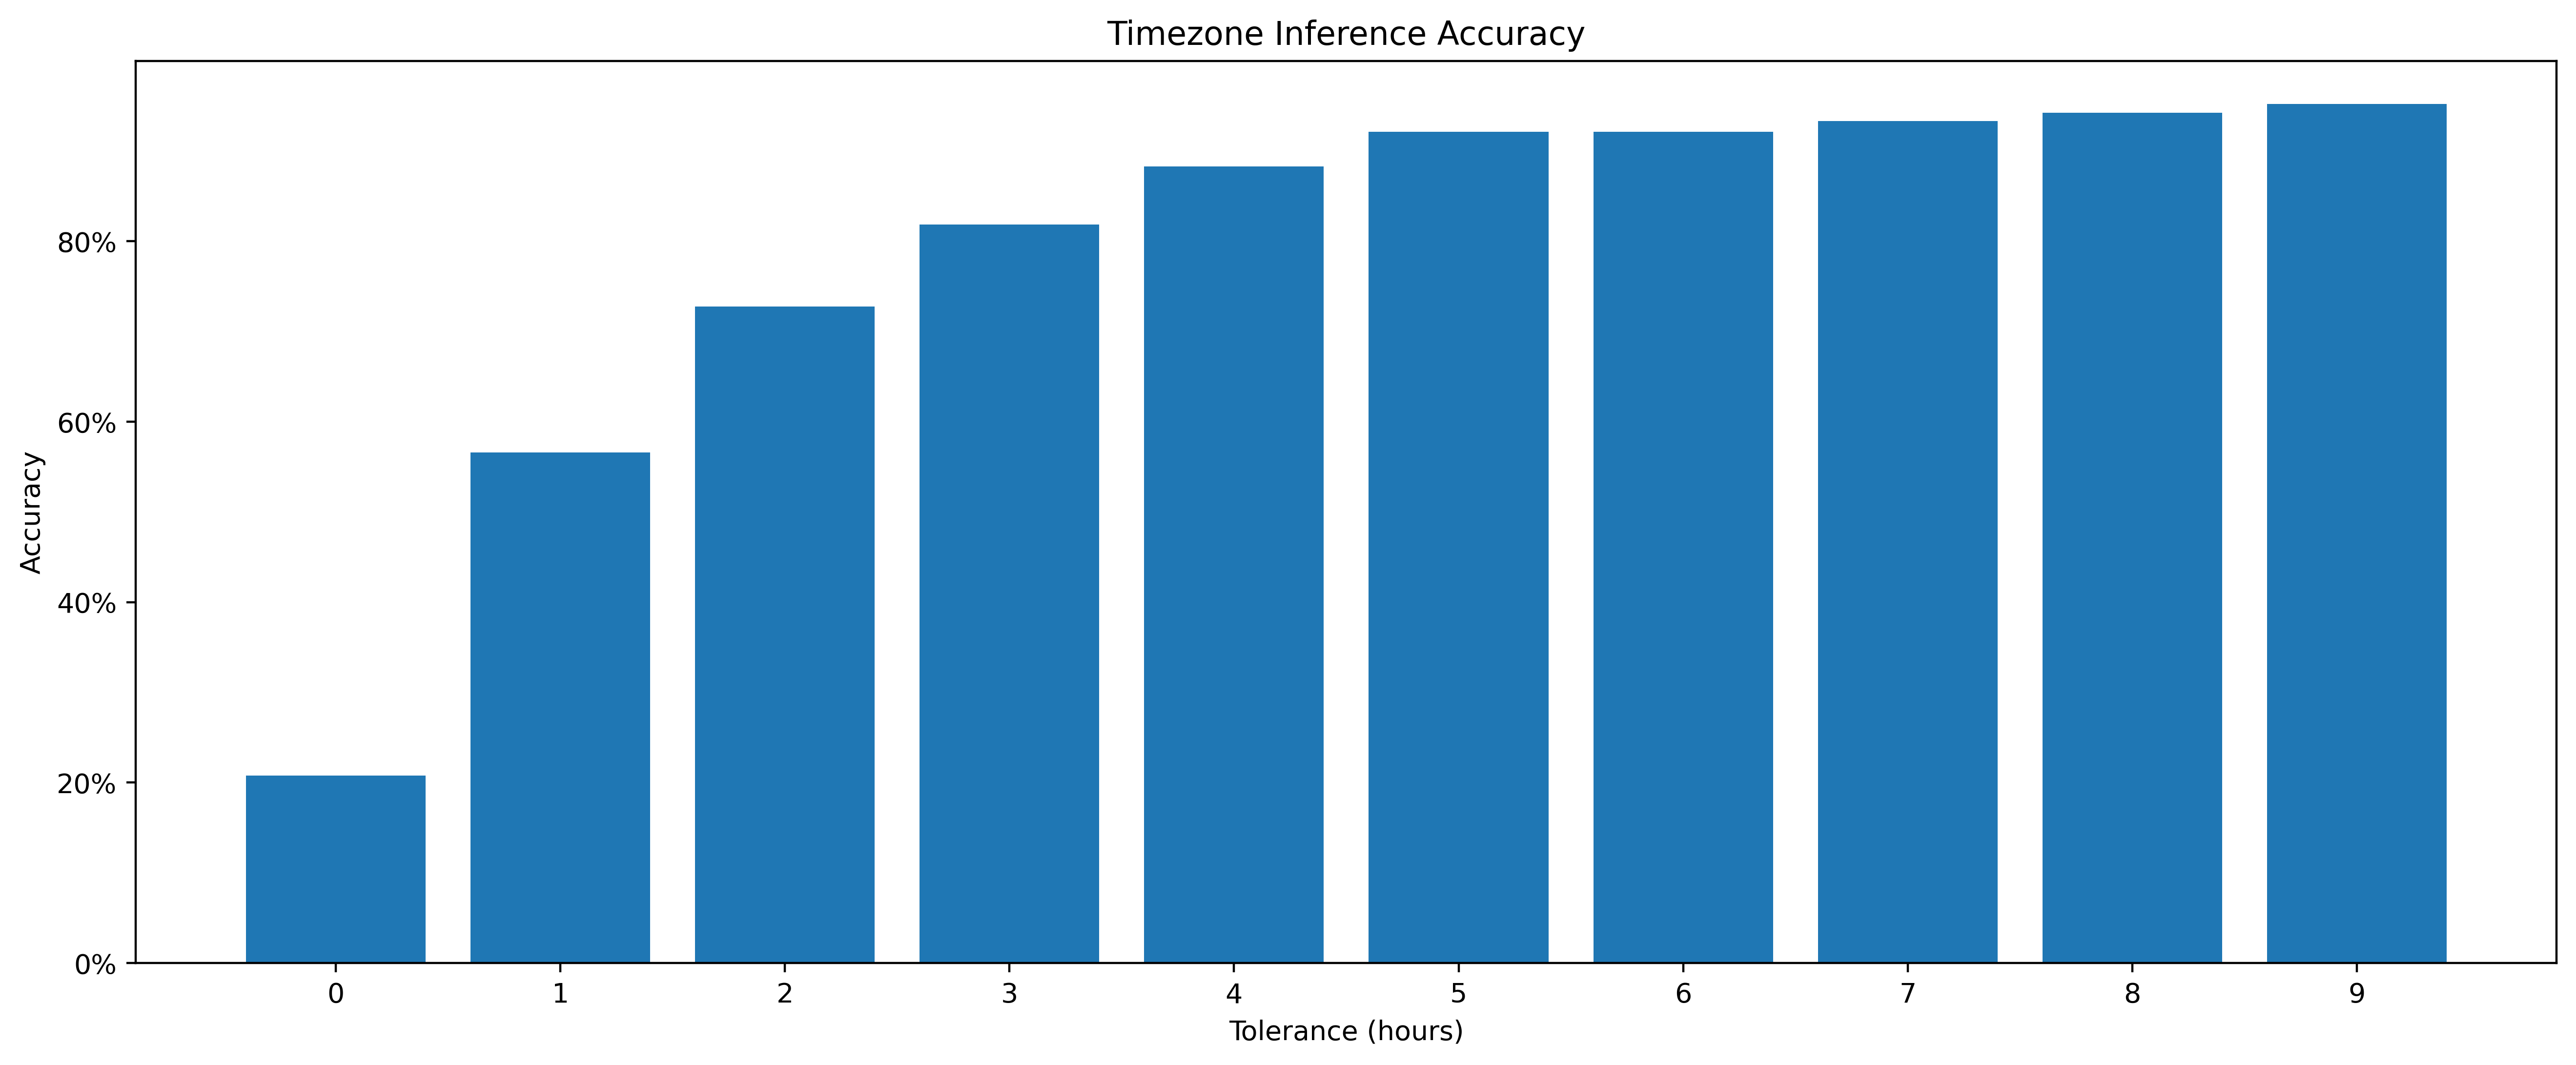
\includegraphics[width=\linewidth]{Images/timezone_inference_accuracy.png}
    \caption{Time zone inference accuracy by tolerance level in hours.}
    \label{fig:time-zones}
\end{figure}

While this method captures general tweeting patterns, it has notable limitations. User behavior varies significantly, and external factors such as work schedules, night shifts, or irregular online habits can distort the assumed daily tweeting rhythm. Additionally, the reliance on mean absolute error assumes that errors in hour misalignment are linearly penalized, which may not always reflect real-world consequences of incorrect time zone estimation.

This approach provides a reasonable approximation of users' time zones when explicit information is unavailable, leveraging behavioral patterns in tweet timing. However, the relatively low exact match rate suggests that further refinement is needed, potentially incorporating additional behavioral signals or machine learning techniques to improve predictive accuracy. These limitations ought to be taken into account when assessing the time of day based results.

For all users without explicit time zone information, the predicted time zone was used for all further analyses.


\subsection{Descriptives}

In total, the sample was made up of 1795 individuals who published 1172 tweets on average (IQR: $422 - 1684$) across the entire time span. Of the individuals for which the gender could be determined, 1218 were female, while only 560 were male. Thus, the dataset was heavily skewed towards women. Approximately 73.61 \% of users in the dataset were younger than 30 years old, with only 10.18 \% being older than 40. 

Demographic information for the users is reported in Table~\ref{tab:descriptives_subset_total}. 

\begin{table}[h]
    \caption{Descriptive statistics for all users included in the analyses.}
    \centering
    
    \begin{tabular}{ccccccccc}
        \hline
        Cohort & n & n female & avg. tweets (sd) & age $\leq 18$ & age $19-29$ & age $30-39$ & age $\geq 40$  \\
        \hline
        Depression & 1270 & 717 & 1182.74 (991.61) & 33.35\% & 40.62 \% & 15.38 \% & 10.53 \% \\
        Anxiety & 492 & 293 & 1169-93 (888.67) & 30.67\% & 41.81 \% & 18.87 \% & 8.65 \% \\
        \hline
    \end{tabular}
    
    \label{tab:descriptives_subset_total}
\end{table}


Most tweets were published during the week days, with Wednesday being the day with the most traffic. Saturday is the day on which the fewest tweets were set off (see Figure \ref{fig:tweets_by_dow}). 

\begin{figure}[h]    
    \centering
    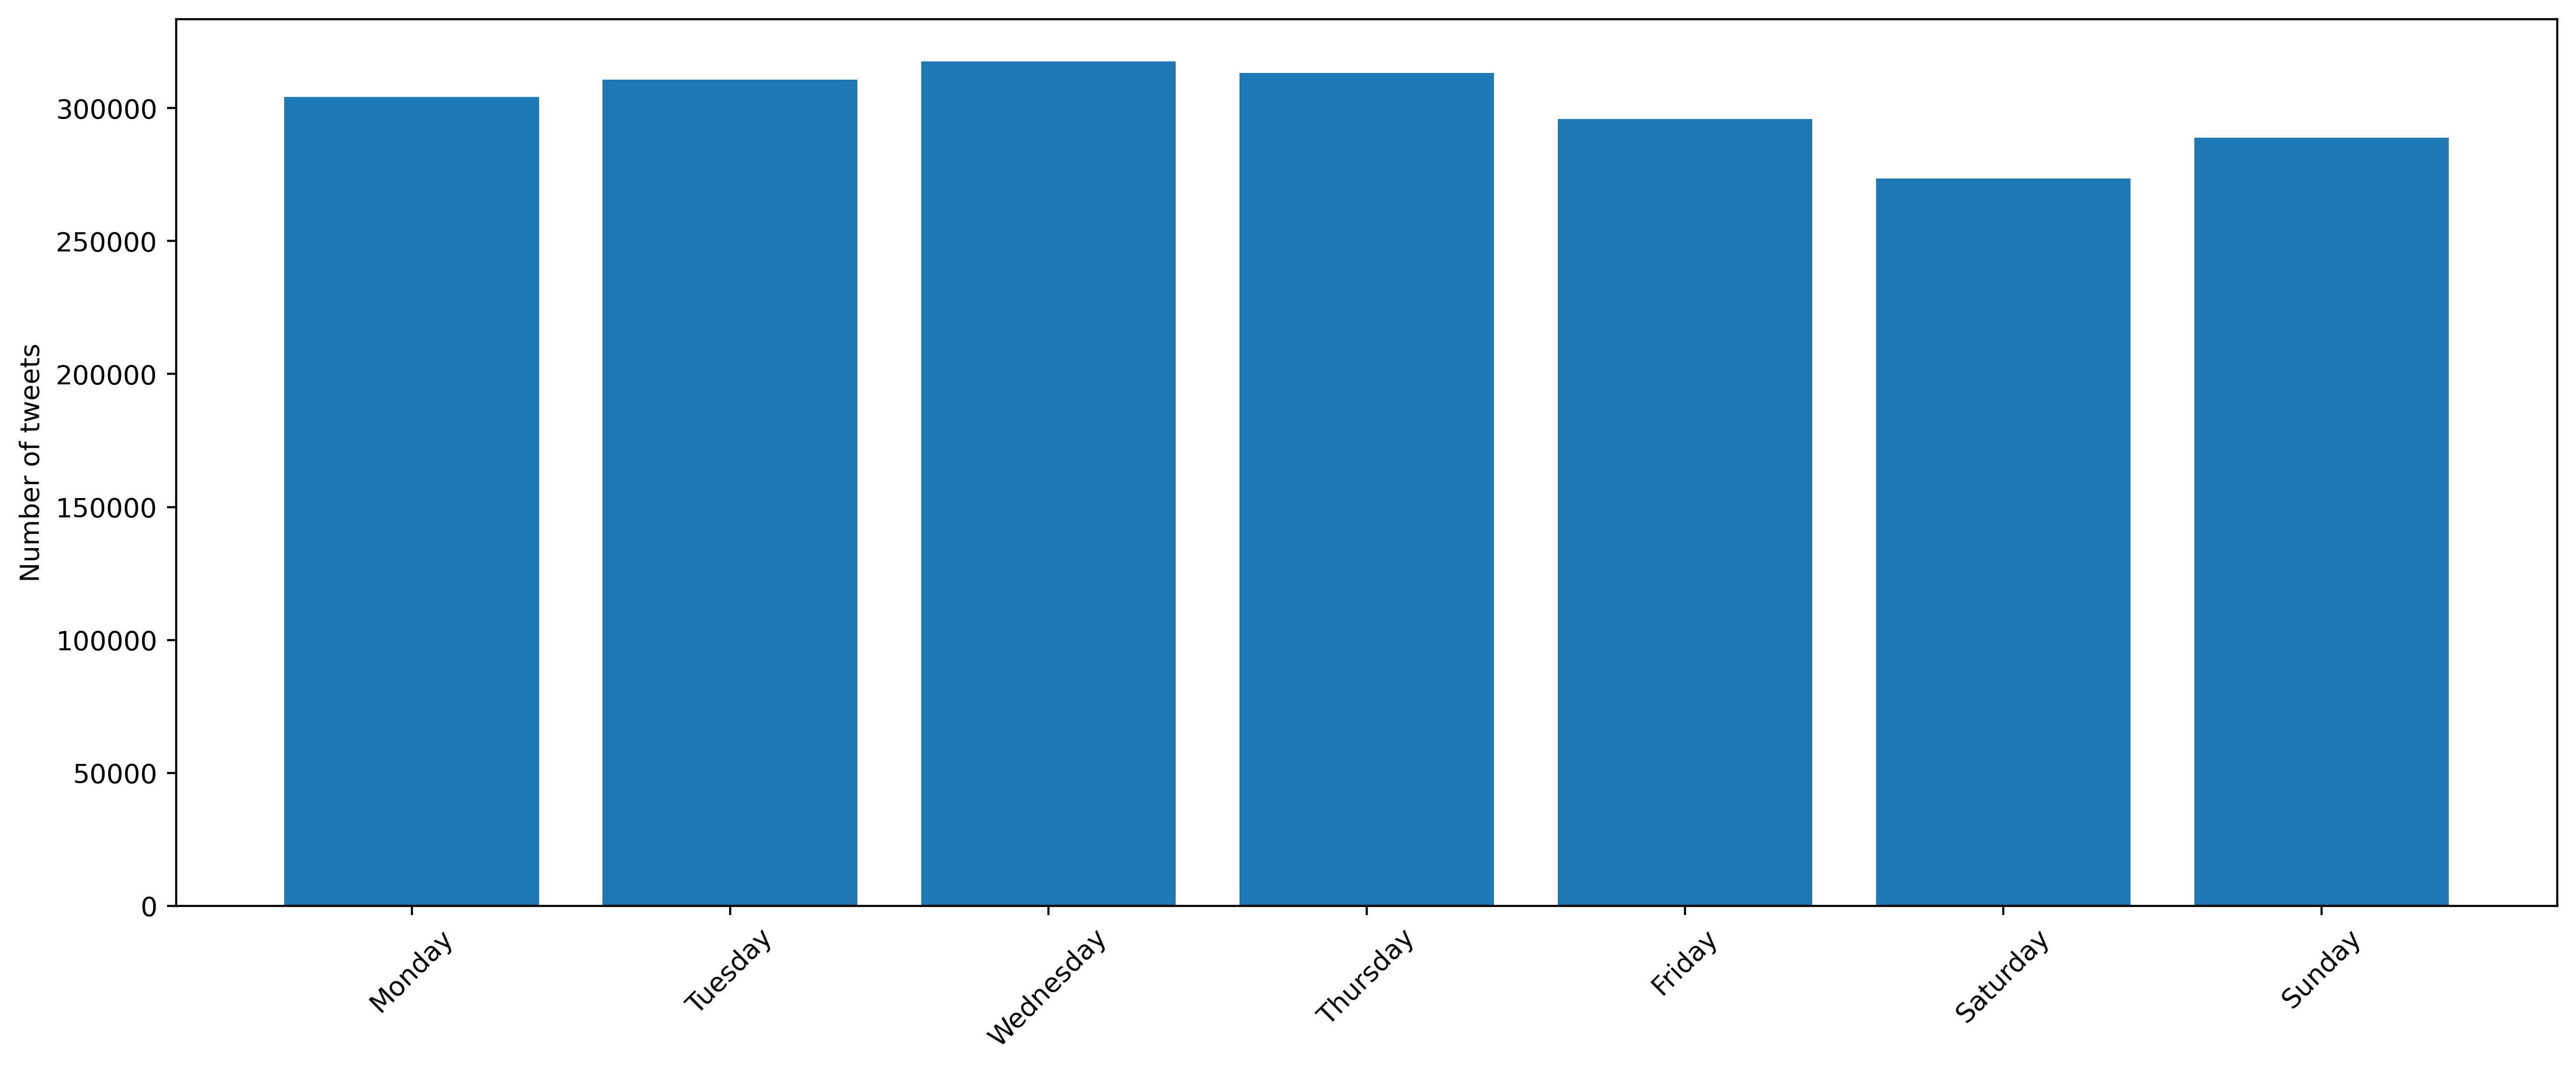
\includegraphics[width=\linewidth]{Images/tweets_by_dow.png}
    \caption{Number of published tweets by day of week}
    \label{fig:tweets_by_dow}
\end{figure}

\begin{figure}[h]
    \centering
    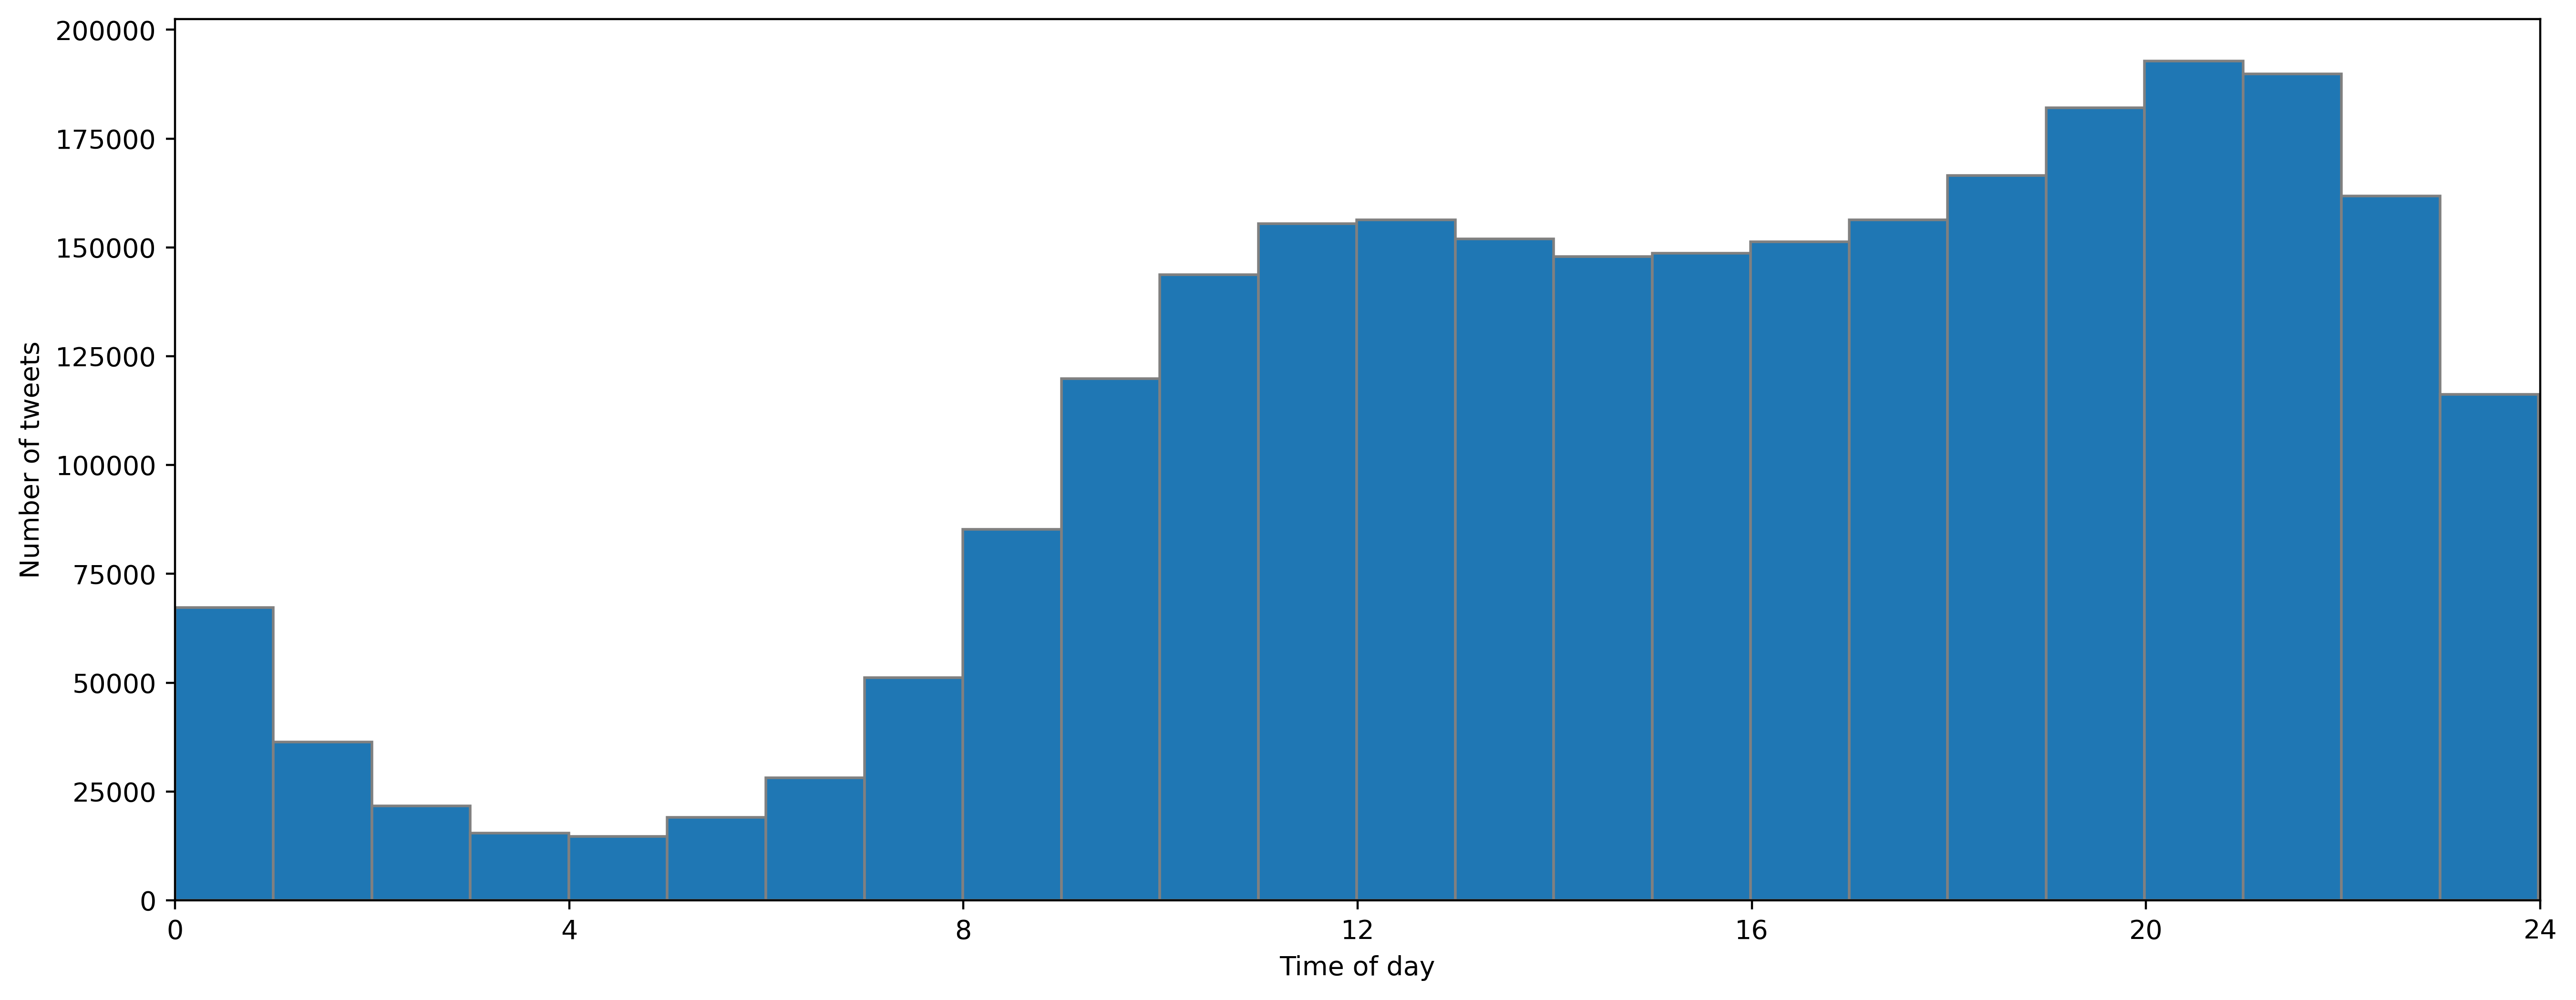
\includegraphics[width=\linewidth]{Images/tweets_per_hour.png}
    \caption{Number of published tweets by time of day}
    \label{fig:tweets_by_tod}
\end{figure}

\begin{figure}[h]
    \centering
    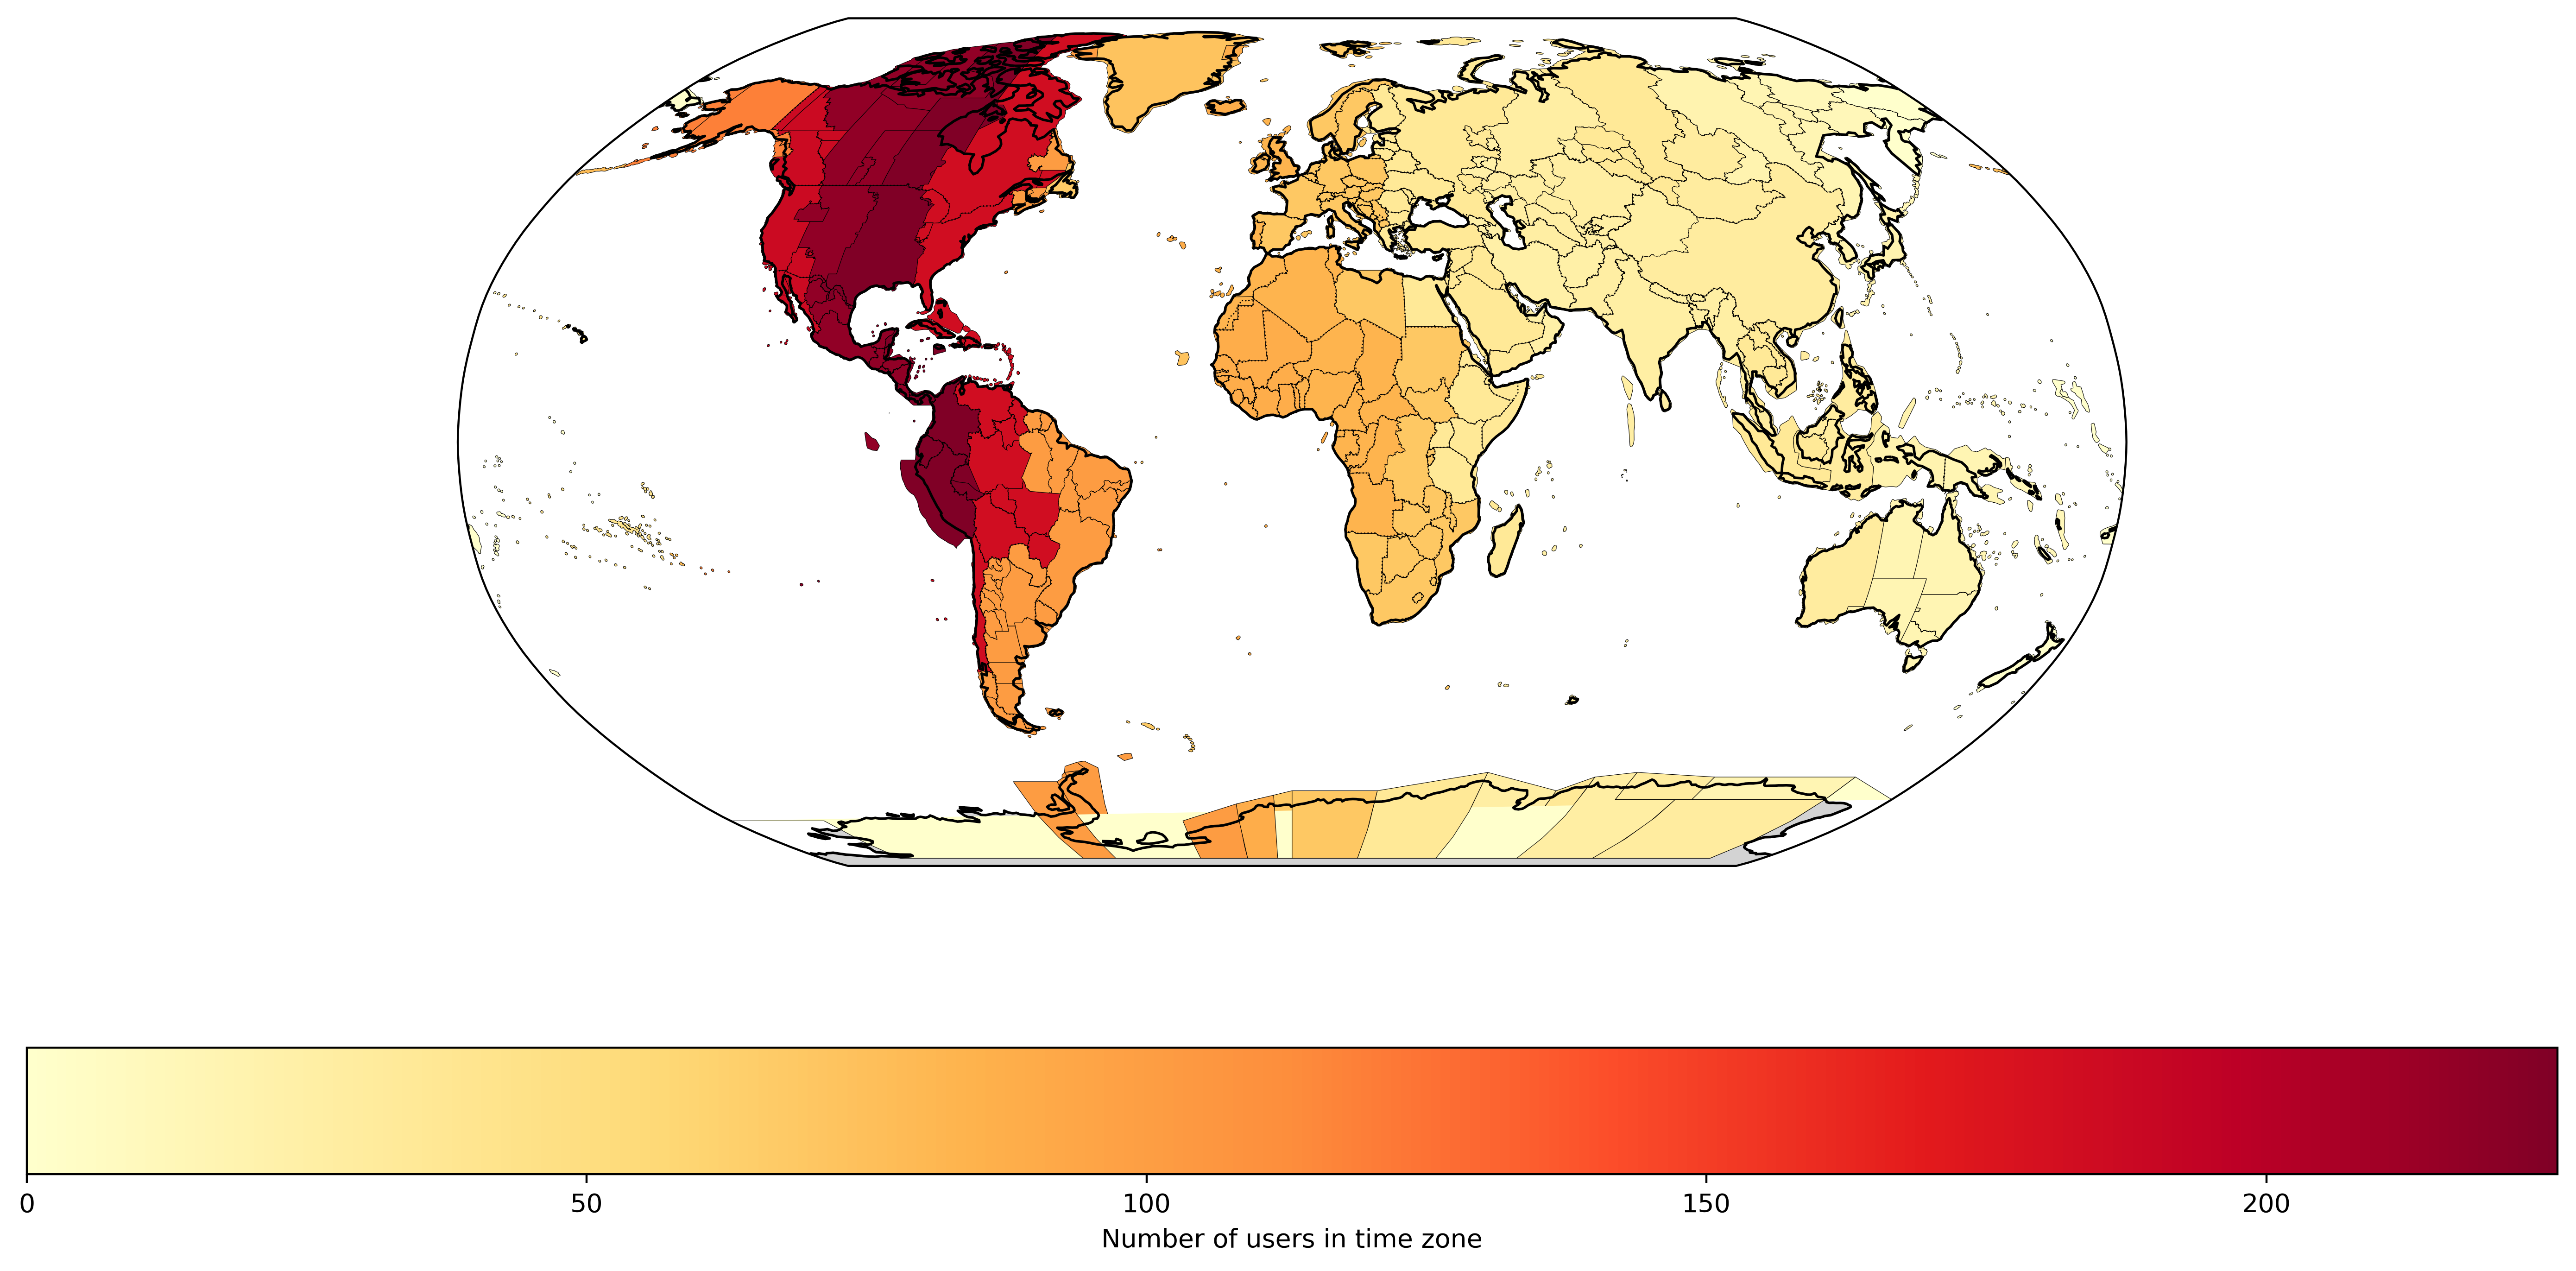
\includegraphics[width=\linewidth]{Images/timezone_frequencies.png}
    \caption{Number of users by time zone}
    \label{fig:timezone_distribution}
\end{figure}

The distribution of Twitter users across time zones, as depicted in Figure~\ref{fig:timezone_distribution}, revealed a clear concentration of users in specific UTC offsets. The map demonstrates a peak in user frequency around UTC \textit{-7} to UTC \textit{-4}, which corresponds to regions such as North America, particularly the Central Time Zones of the United States. A secondary concentration is observed around UTC \textit{0}, likely reflecting users from Western Europe. There appears to be little activity in Asia, indicating that most activity originated in the western hemisphere. This uneven distribution highlights the geographical bias in Twitter activity, which should be considered when analyzing temporal trends in sentiment or online behavior. This was likely influenced or even caused by filtering for English-only tweets.

\section{Methods}
\label{sec:methods}

For all statistical significance tests, a significance level of $0.05$ was assumed.

\subsection{Overall measurements of negative affect and its variability}

As proposed in \citet{rutter2024}, one way of estimating negative affect levels and variability is, to simply aggregate all observations for an individual to compute a single score for them. Thus, for investigating NA levels, one takes the arithmetic mean of all NA scores for a person and for NA variability one takes the standard deviation of all NA scores for that person.

This yields an overall NA level $x_i$ and an overall NA variability $\sigma_i$ for each person $i$. Then, let $A$ be the set of anxiety patients and $D$ the set of depression patients. 

Then, the separate overall mean NA level scores are

\begin{equation}
    \bar{x}_a = \frac{\Sigma_{i = 1}^{n} x_i}{n}, n := |A|
\end{equation}

for the A cohort and 

\begin{equation}
    \bar{x}_d = \frac{\Sigma_{i = 1}^{n} x_i}{n}, n := |D|
\end{equation}

for the D cohort. Similarly, the separate overall mean NA variability scores are

\begin{equation}
    \bar{\sigma}_a = \frac{\Sigma_{i = 1}^{n} \sigma_i}{n}, n := |A|
\end{equation}

for the A cohort and 

\begin{equation}
    \bar{\sigma}_d = \frac{\Sigma_{i = 1}^{n} \sigma_i}{n}, n := |D|
\end{equation}

for the D cohort.

Then, one can compare the two means and make inference regarding the differences on the population level by testing the null hypotheses

\begin{equation}
    H_{0V} : \bar{\sigma}_a = \bar{\sigma}_d
\end{equation}

and

\begin{equation}
    H_{0L} : \bar{x}_a = \bar{x}_d.
\end{equation}

\subsection{Localized measures of negative affect and its variability}

In order to obtain localized measures of negative affect magnitude and variability, indicators were computed in rolling windows across the time series. Thus, for each individual, there was not just one overall affect level, but instead one for each smaller time period. After obtaining these mean NA levels for each window, the aggregated scores from all windows for an individual were further aggregated. For assessing NA levels, they were again averaged, while the standard deviation of these scores represents the overall NA variability for an individual. The window construction is illustrated in Figure \ref{fig:windowing}

The first window size option was a 6-hour window. We aimed to capture a more stable estimation of short-term affect levels. The threshold of 6 hours was chosen because it is not too short where it would merely capture single tweets, but also short enough in order to capture short-term affect levels. Each observation served as the center of a window exactly once. Thus, for each observation in the dataset, a window of three hours before and three hours after the observation was created and the NA levels were aggregated using the arithmetic mean in order to obtain a window score. If only one observation was contained in a window, the window centered around it was omitted for all analyses. 

The second window size that was tested is a daily aggregation. For this, all observations for a person from a single calendar day were aggregated. We assumed that users' NA levels do not just fluctuate during the day, but also between days. This aimed to operationalize the idea of "good" and "bad" days. Thus, we obtained a single NA score for each calendar day, represented by the mean NA score of all tweets on that day.



\begin{figure}[h]
    \centering
    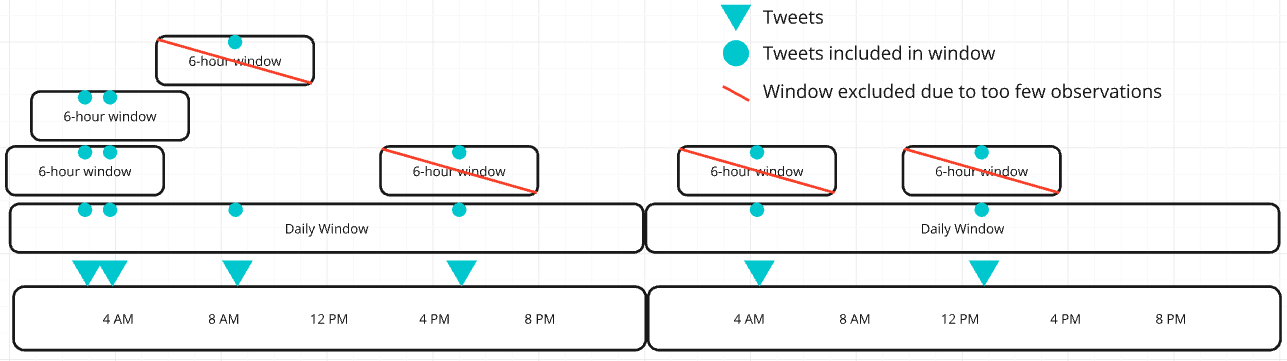
\includegraphics[width=\linewidth]{Images/windowing.png}
    \caption{Construction of windows on tweets of a single individual}
    \label{fig:windowing}
\end{figure}

\subsection{Validity of application of simple aggregation functions}

For windowed analyses, all observations for a person within a certain time window (which yield a distribution of NA values) were aggregated to a single number. For NA levels, the arithmetic mean was used, while NA variability was measured by standard deviation. These measurements, albeit simple, put some assumptions on the data that required investigation. 

First, the mean of a distribution always gives the average value of all observations, can be inflated by outlier observations quite easily though. Therefore, its interpretation can change for skewed distributions because there no longer is such a clear center of the distribution as in a symmetric one. The mean $\bar{x}$ of a sequence $X$ is defined as 

\begin{equation}
    \bar{x}= \frac {1}{n} \sum _{i=1}^{n}x_{i},
\end{equation}

while the sample standard deviation $\sigma$ is

\begin{equation}\sigma
 = \sqrt\frac{\sum{(x_i-\bar{x})^2}}{n-1}.
\end{equation}

It becomes clear, that $\sigma$ depends on $\bar{x}$ and therefore has the same interpretation assumptions. It follows, that the standard deviation is a measure of symmetric spread around the mean and also suffers from the same susceptibility to outliers that the arithmetic mean suffers from.

Whether this is a good measure of aggregation depends on a few facts about the distributions. Figure \ref{fig:suitability_mean} shows three types of distribution that have very different characteristics.

\begin{figure}[h]
    \centering
    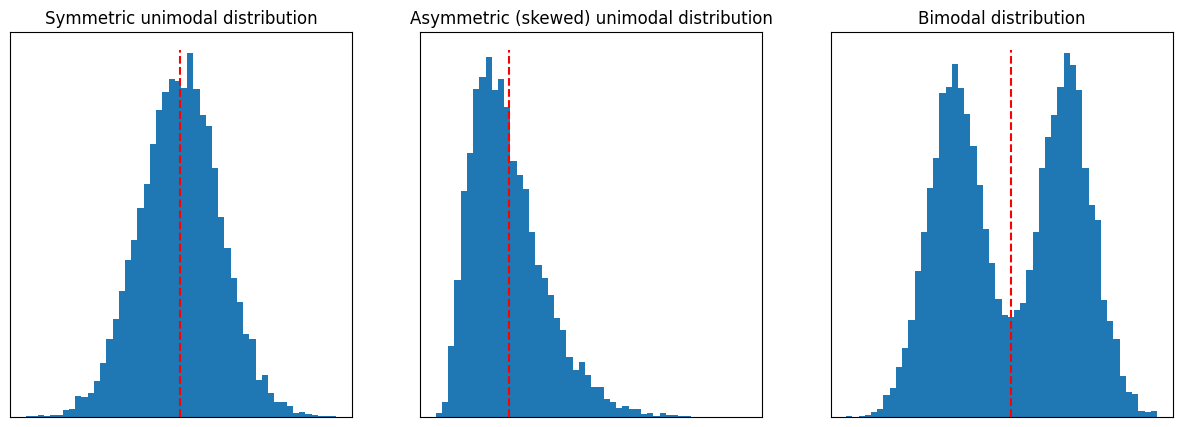
\includegraphics[width=\linewidth]{Images/suitability_of_mean_agg.png}
    \caption{Visualization of placement of arithmetic mean (red dashed lines) for different types of distribution}
    \label{fig:suitability_mean}
\end{figure}

First, the symmetric unimodal distribution can be summarized quite well using an arithmetic mean (as indicated in the figure). In this case, the mean, mode and median are all approximately equal. Also, its standard deviation gives a very good estimate of spread, because the observations are evenly spread around the mean. This is because the standard deviation is approximately just the mean squared deviation from the sample mean and therefore symmetric.

Second, the asymmetric, or skewed, distribution shows a different behaviour. In this case, the mean is not at the peak of the distribution (mode), indicating that it is not necessarily the perfect means of assessing location of the distribution. One could debate here, whether the mean is what we intend to measure or whether one is rather interested in the mode of the distribution.

Third, the bimodal distribution represents an entirely separate challenge. It is (in the case from Figure \ref{fig:suitability_mean}) made up of two symmetric unimodal distributions that are displaced by some offset. In this case, if both distributions are equal in spread and simply placed at different points on the x-axis, the placement of the mode of this distribution is simply a random coin toss between the two modes of the underlying distributions. The mean will always measure some point in between both modes. In this case, one could argue that neither the mode, nor the mean, nor the median is a good measure of location, because the distribution is likely not one, but multiple that might even be separable by some criterion.

Because the quality and interpretation of the aggregation of observations for a person within a window depend so much on the kind of underlying distribution, we had to investigate the distributions. Since the ideal case (in which the mean is basically a perfect measure of NA level) is the symmetric unimodal distribution, a test was performed in order to check whether this assumption holds. 

For this test, all means and medians of these distributions (for one person, for one window) were gathered and compared using a pair-wise t-test for dependent samples. This tests the means and medians for equality. If they are unequal, there must be some systematic skewedness in the data, indicating that the applicability of the mean and standard deviation as aggregation measures is debatable.

The results of this analysis showed, that for the raw data ($t(1301) = 106.68; p < .001$), the 6-hour windowed NA levels ($t(1298) = 32.72; p < .001$) and the daily aggregation ($t(1301) = 37.17; p < .001$), the assumptions were violated. Thus, there is reason to believe that mean and standard deviation were not an optimal measure of location or spread of the NA distribution. 

\subsection{Group comparisons with localized measurements}

As described, all window aggregations for a person were aggregated to obtain a single score for a person. This score was either the mean (for NA level comparisons) or the standard deviation (for NA variability comparisons) of windowed NA levels. Thus, each participant was represented by a single value on both dimensions (NA level and NA variability).

With these scores for each individual, they were again split into anxiety and depression cohorts. Then, the two samples were compared with respect to their means using Mann-Whitney-U tests. Thus, for NA level comparisons, the mean NA levels for each user were compared, while the mean standard deviation was compared for NA variability. The obtained test statistic was tested for statistical significance and used for inference.

\subsection{Analysis of negative affect differences using linear mixed models}

In addition to the overall and windowed aggregations of NA levels and NA variability, we introduce a new method for inferential statistics. Here, linear mixed models (LMM) were used to model the correlation between NA scores and a set of predictor variables. In this approach, NA level differences as well as NA variability differences between the cohorts can be extracted from a single process.

The assumption that underlies this method is, that the lower the affect variability, the easier it should be to predict the negative affect level at a given time. So, in order to test whether there are differences in variability between cohorts, the residual variances of a predictive regression model can be compared. If one cohort has higher residual variance than another, one can conclude, that the affect levels are more difficult to predict and therefore higher in variability.

With this method, one can estimate the differences in variability that are not simply due to external factors, but seemingly unexplainable. This is because one can include external factors in the form of covariates in the model specification, yielding a more robust estimation of variability differences.

The dataset consisted of repeated measures of sentiment (VADER NA score) for multiple users over time, alongside other covariates (user-level features). Since sentiment was tracked across time, the dataset was inherently longitudinal, where series of observations are nested within individuals.

In this type of data, several key challenges arise. One challenge is correlation within subjects. Repeated observations of the same user are not independent. Responses (VADER scores) for a given user are likely correlated over time. Failing to account for this correlation may lead to biased standard errors and incorrect inference. 

Another challenge is that users can be quite heterogeneous with regards to the outcome variable and its dependence on covariates. Each user may have unique, unobserved characteristics (e.g., gender, age, baseline sentiment levels) that affect their sentiment trajectory. Ignoring this variability can lead to biased coefficient estimates.

\subsubsection{Linear Mixed Modeling}

A linear mixed model (LMM) is a robust solution for this type of structured data. One of the key reasons for using it is that LMMs introduce so-called random effects, which allow for modeling user-specific intercepts and/or slopes. These are extra terms that are added to the model formula, accounting for the unobserved heterogeneity across users. In this case, it can model how different users have different baseline levels of sentiment or respond differently to covariates.

Linear mixed models (LMMs) extend traditional linear regression by incorporating both \textit{fixed effects} and \textit{random effects}. A standard linear regression model assumes that the response variable $y_i$ for subject $i$ is modeled as:
\begin{equation}
    y_i = \beta_0 + \beta_1 x_{i1} + \dots + \beta_p x_{ip} + \epsilon_i,
\end{equation}

where $\beta_0, \beta_1, \dots, \beta_p$ are the fixed coefficients and $\epsilon_i \sim \mathcal{N}(0, \sigma^2)$ is the error term.

In contrast, an LMM incorporates random effects to account for variability within groups or subjects. The model for repeated measures or hierarchical data is given by:
\begin{equation}
    y_{ij} = \beta_0 + \beta_1 x_{ij1} + \dots + \beta_p x_{ijp} + u_i + \epsilon_{ij},
\end{equation}

where $y_{ij}$ is the response for subject $i$ at time $j$, $u_i \sim \mathcal{N}(0, \sigma_u^2)$ is the random effect specific to subject $i$, and $\epsilon_{ij} \sim \mathcal{N}(0, \sigma^2)$ is the unexplainable random variability.

This is what allows the model to deal with the aforementioned challenges of panel data. Specifically, including a random intercept allows the model to account for individual-specific deviations from the population average, thus better capturing the sentiment variations across users.

Given the nature of the data and task at hand --- predicting user sentiment (VADER NA scores) over time based on covariates --- an LMM provides:
\begin{itemize}
    \item A means of handling the hierarchical structure of the data (users, repeated observations).
    \item The ability to partition variance into \textit{within-subject} (temporal changes) and \textit{between-subject} (user-level) components.
    \item Robust handling of correlated observations and unobserved user heterogeneity, which are central concerns in this context.
\end{itemize}

\subsubsection{Modeling and feature engineering}


%%%%%%%%%

To investigate temporal effects at varying granularities, the LMM approach was applied separately to two of the three different temporal resolutions of the data: unaggregated (per-tweet) and 6-hour windows. Each resolution was modeled independently to allow for the detection of patterns that may vary depending on the temporal scale. In the unaggregated case, the outcome was the raw per-tweet value, while it was the aggregated mean NA level for the windowed approaches.

In order to preserve temporal coherence between the outcome and the covariates, all predictor variables were extracted from the tweet located at the temporal center of each window—i.e., the tweet closest to the midpoint in time. This procedure ensured that the covariates used in the model are representative of the window in which the outcome is computed, without introducing look-ahead bias or artificial lag effects. This was essentially the same procedure as for calculating outcomes.

To obtain robust and interpretable parameter estimates, a set of relevant covariates was included in the modeling process. Demographic information about the user was incorporated through two features: a binary indicator of predicted gender, and a categorical variable representing the user’s age group, binned into discrete intervals. These variables helped account for differences in linguistic behavior and platform engagement across demographic segments. In addition, a binary variable was used to indicate whether the tweet (or center tweet in the window) was posted on a weekend (Saturday or Sunday), capturing behavioral differences that may occur between weekdays and weekends.

Temporal variation within a single day was modeled using a spline-based representation of the time of day at which the tweet was posted, expressed in continuous hours from 0 to 24. This representation allowed the model to capture smooth, nonlinear trends that may influence the outcome variable throughout the day. For windowed data, the spline eas computed using the timestamp of the center tweet. This spline-based time-of-day feature was included in both temporal resolutions.

The spline functions used in this analysis were piecewise polynomial curves joined at specified knot points. The flexibility of the spline representation was determined by three parameters: the number of knots, the placement of the knots along the 24-hour time axis, and the degree of the polynomial segments. These parameters were optimized by minimizing the root mean squared error (RMSE) under a 5-fold cross-validation procedure carried out on the entire dataset. The 5-fold cross validation was chosen in order to reduce bias that comes with testing model fit on the training set. The spline configuration with the lowest cross-validated RMSE was then fixed and applied consistently in the corresponding models.

RMSE is defined as 

\begin{equation}
    \mathrm{RMSE} = \sqrt{\frac{\Sigma_{i=1}^N (y - \hat{y})^2}{N}},
\end{equation}

where $N$ is the number of samples, $y$ the true outcomes, $\hat{y}$ the predicted outcomes. Thus, it represents a metric for gauging the predictive performance of a regression model.


Knot placement was defined to be equidistant (for two knots, they would be placed at 8 AM and 4 PM) and knot count was varied between two and five. The polynomial degree was varied between two and three. This spline fit optimization process was adapted to this context from a different study that also aimed to fit basis splines to time series data \citep{octpaper}.



Finally, the model included an autoregressive term on the NA score, representing the previous NA score for each observation. This aimed to model the correlation between emotional valences of successive tweets (or periods). Therefore, the model was able to capture the idea that successive tweets are likely to have similar levels of affect. It must be noted, that times between tweets were naturally not constant. Since the autoregressive term was included as a linear predictor variable in a linear regression model, we assumed that its effect is independent of the time between tweets. This is potentially a very strong assumption, since it appears reasonable that autocorrelation between tweets is highest when multiple tweets occur in a short time span.

%Since this is likely to be more effective when a tweet is issued shortly after the previous one, the autoregressive term is used as part of an interaction between the previous VADER score and the time that expired after the previous tweet. 
Additionally, it was assumed, that NA levels decrease over time if there has not been a tweet for a long time. Therefore, the model included the time that passed since the last tweet (or period) in seconds as predictor variable.
Since the time between successive tweets was highly skewed, it was log-transformed to achieve a more balanced distribution. This must be taken into account when interpreting regression coefficients.

\subsubsection{Model fit assessment}

In order to gauge how well the LMM fit the data, there are a few metrics to be considered. First, as used for spline fits, RMSE can be used for obtaining a general measure of prediction accuracy. Another metric that can be highly useful in determining predictive performance is the coefficient of determination ($R^2$). $R^2$ represents the proportion of variance that is explained by the proposed model, which would not be explained by a \textit{null} model. This \textit{null} model is the most basic model possible. In the case of simple linear regression, this is mostly an intercept-only model. Thus, this \textit{null} model simply predicts the sample mean for all samples. $R^2$ can be defined as

\begin{equation}
    R^2 = 1 - \frac{RSS}{TSS},
\end{equation}

where $RSS$ is the residual sum of squares, while $TSS$ is the total sum of squares. $RSS$ is thus simply the variance of the residuals of the proposed model. $TSS$ represents the variance of the residuals of the \textit{null} model.

Since the LMMs do not only include fixed effects like OLS regressions do, an adjusted version of $R^2$ is used \citep{nakagawa2013general}. This is called conditional $R^2$ and takes into account the predictive performance of the entire model, thus meaning random as well as fixed effect terms. This gives a good indication for how well the model fits the data and to what extent it is able to predict real-world NA levels from the available predictors.


\subsection{Robustness checks}

In order to analyze, how reliant the results are on assumptions, the analyses were run in different scenarios. First, VADER was replaced as sentiment analysis tool. Second, the applicability of the method to bounded distributions was assessed. 

%First, all analyses are also re-run with aggregated VADER compound scores, which do not give an estimate of negative affect levels, but rather of overall affect. Thus, also positive keywords are taken into account and the compound score is inverted to again be an indicator of negative affect levels.



%Using the VADER NA scores yields a highly zero-inflated distribution, as can be seen in Figure \ref{fig:vader_hist_entire_sample}. The analyses are re-run, removing all NA scores of 0, because this is indicative of simply the absence of VADER-related keywords in the tweet. Therefore, a dataset is obtained that contains only observations that show evidence of negative affect. The goal is, that this yields a more balanced outcome variable. It is important to note though, that observations without VADER keywords are not necessarily void of meaning, but could also encode positive or neutral affect.



\subsubsection{Transformer-based sentiment}

In addition, to address several known limitations of the VADER sentiment analysis tool, the analyses were replicated using sentiment estimates obtained from a transformer-based language model specifically trained on Twitter data. While VADER is a popular lexicon-based approach for sentiment analysis in social media contexts, it relies on predefined word lists and simple rules, making it less sensitive to linguistic nuances such as sarcasm, slang, or context-dependent meaning — all of which are highly prevalent in user-generated content like tweets. Moreover, VADER operates independently of word order and syntax, which can further limit its ability to accurately capture the affective tone of more complex text.

To overcome these limitations, a transformer-based sentiment classifier was employed. It is a RoBERTa \citep{liu2019roberta} model, that represents an extension on the basic BERT \citep{devlin2019bert} model. The model was trained on ~124M tweets from January 2018 to December 2021, and finetuned for sentiment analysis, producing probabilistic outputs for negative, neutral, and positive sentiment categories \citep{cardiff_sentiment}. 

For the purposes of the present analyses, the probability assigned to the negative class was used as a continuous measure of NA, reflecting the model’s estimation of negativity in the text.

Due to the considerable computational demands of applying the transformer-based model to the entire dataset, the analyses were performed on a representative subset of the data. Specifically, 230 users were randomly sampled from each of the anxiety and depression cohorts, ensuring balanced group sizes and facilitating direct comparisons. The members of the A cohort were then matched with their best match from the D cohort, depending on the similarity of their tweet frequency (thus, each A cohort member received a best D cohort partner, depending on how many tweets they created in the time span).

Descriptive statistics for these sub-samples are reported in Table~\ref{tab:descriptives_subset_roberta}. 

\begin{table}[h]
    \caption{Descriptive statistics for sub-sample with generated RoBERTa NA scores.}
    \centering
    
    \begin{tabular}{ccccccccc}
        \hline
        Cohort & n (sd) & n female & avg. tweets & age $\leq 18$ & age $19-29$ & age $30-39$ & age $\geq 40$  \\
        \hline
        Depression & 230 & 146 & 1030.18 (726.66) & 28.46\% & 41.09 \% & 17.43 \% & 13.02 \% \\
        Anxiety & 230 & 163 & 1085.86 (757.09) & 24.66\% & 42.36 \% & 23.37 \% & 9.61 \% \\
        \hline
    \end{tabular}
    
    \label{tab:descriptives_subset_roberta}
\end{table}

This sampling strategy provided an efficient yet robust approach to exploring potential differences in NA levels while leveraging the enhanced capabilities of a context-aware sentiment analysis model.

After obtaining the RoBERTa-derived NA scores, we used them to evaluate whether significant differences in NA levels and variability persist between the A and D cohorts, even when applying an alternative sentiment analysis method. To this end, we conducted Mann-Whitney U tests on within-person means and standard deviations across the full time series. We also fit a LMM, following the previously described specification, to the data segmented into 6-hour windows. This approach provided a comprehensive assessment of whether the findings based on VADER sentiment analysis are robust to potential limitations inherent in the VADER methodology.

The distribution of NA scores derived from the RoBERTa model differed substantially from that of the VADER model. As shown in Figure \ref{fig:vader_roberta_hist}, the RoBERTa NA scores exhibited a bimodal distribution, with a pronounced peak at the lower end of the scale (near 0) and a secondary rise in density toward the upper end (near 1). This suggests that the RoBERTa model frequently assigned either very low or very high NA scores, with fewer scores in the mid-range. In contrast, the VADER NA scores followed a strongly right-skewed unimodal distribution, with the vast majority of observations concentrated near zero and a rapid decline in density as scores increase.

While both models generate scores across the full 0–1 range, RoBERTa appeared to make broader use of the scale, particularly in the upper half. VADER, by comparison, predominantly assigned low NA values, with scores above 0.5 being rare. This indicates that RoBERTa may be more sensitive to high-intensity negative sentiment, whereas VADER may systematically underrepresent such cases.

These distributional differences have important implications for downstream analyses. RoBERTa’s broader score dispersion and greater frequency of high NA values suggest that it may better capture variability in negative affect, particularly at the higher end of the spectrum. In contrast, the conservative scoring pattern of VADER may introduce a floor effect, limiting its sensitivity to subtle or severe expressions of negative emotion.


\begin{figure}[h]
    \centering
    
\includegraphics[width=\linewidth]{Images/roberta_vader_distribution.png}
    \caption{Distribution of VADER and RoBERTa NA scores across the entire dataset.}
    \label{fig:vader_roberta_hist}
\end{figure}

\subsubsection{Testing validity of analyzing bounded distributions}

The empirical data for this study originated from bounded distributions, and the means and standard deviations of two samples were compared. However, this approach can be problematic due to the intrinsic statistical dependence between the mean and the standard deviation in such distributions. Specifically, for bounded distributions, such as VADER NA scores (bounded between 0 and 1), the standard deviation is not independent of the mean. Instead, it is typically a function of the mean, with variability often peaking at intermediate values and decreasing near the bounds.

This inherent mean-variance coupling implies that observed differences in standard deviation may be partially or wholly attributable to differences in means, rather than reflecting distinct dispersion structures across groups. Consequently, simultaneous interpretation of changes in both parameters may lead to misleading conclusions, particularly if inferential statistics are applied without adjusting for this dependence.

As a robustness check to address the inherent dependency between the mean and standard deviation in bounded distributions, a sub-sampling procedure was performed in which pairs of users were constructed from the two cohorts such that their means were nearly identical. By holding the means constant across sub-samples, this approach aimed to isolate differences in variability that are not confounded by shifts in central tendency. 

The pairs consisted of one anxiety patient and one depression patient each. Their average NA level across the entire time series was computed. Since the depression cohort was overall the smaller one, each depression patient was assigned a "best-fitting" anxiety patient. In order to further improve the robustness of this method, the pairs for which the mean difference was among the highest 20\% were omitted. This left 648 highly similar pairs of users with negligible mean NA differences.

Then, the standard deviations of these matched sub-samples were compared to assess whether differences in dispersion persist independently of the mean, thereby providing a more reliable inference about group-level variability. In order to provide solid inferential information, a Mann-Whitney-U test was run to test the differences for statistical significance. If the result supports the hypotheses, that indicates that the bounded distributions are not a significant limitation to the study to the extent that they would invalidate the results.

The same analysis was also performed for the RoBERTa based NA scores to test the validity of that approach as well.

\section{Results}
\label{sec:results}

In order to answer the posted research questions, the results from the aforementioned analyses are described in this section.

\subsection{Simple comparisons}

In this section, the results from simple two-sample comparisons between the two cohorts are presented. Each type of aggregation is shown separately.

\subsubsection{Overall aggregated measures}

To assess baseline differences in affective expression between clinical groups, we first examined overall NA levels and their variability across the entire time series. A Mann-Whitney U test confirmed a significant difference in mean NA levels between the depression and anxiety cohorts ($U = 227445$, $p < .001$). Individuals diagnosed with depression exhibited higher average NA levels ($M = 0.0878$) compared to those in the anxiety cohort ($M = 0.0844$). This result suggests that, on average, individuals with depression report more pronounced negative affect throughout the study period than those with anxiety.

In addition to absolute NA levels, we also investigated the variability of negative affect, operationalized as the standard deviation of NA scores across the full time series for each individual. Again, a significant difference was observed ($U = 237172$, $p < .001$), with the depression cohort displaying greater affective instability. Specifically, the mean standard deviation of NA scores was $0.1356$ in the depression cohort, compared to $0.1276$ in the anxiety cohort. This finding suggests that individuals with depression not only experience more intense negative affect but also exhibit more fluctuations in their emotional state over time.

These results, visualized in Figure \ref{fig:overall_histograms}, provide strong evidence that depression is associated with both higher levels and greater variability of negative affect when examined across the entire observational window. 



\begin{figure}[h]
    \centering
    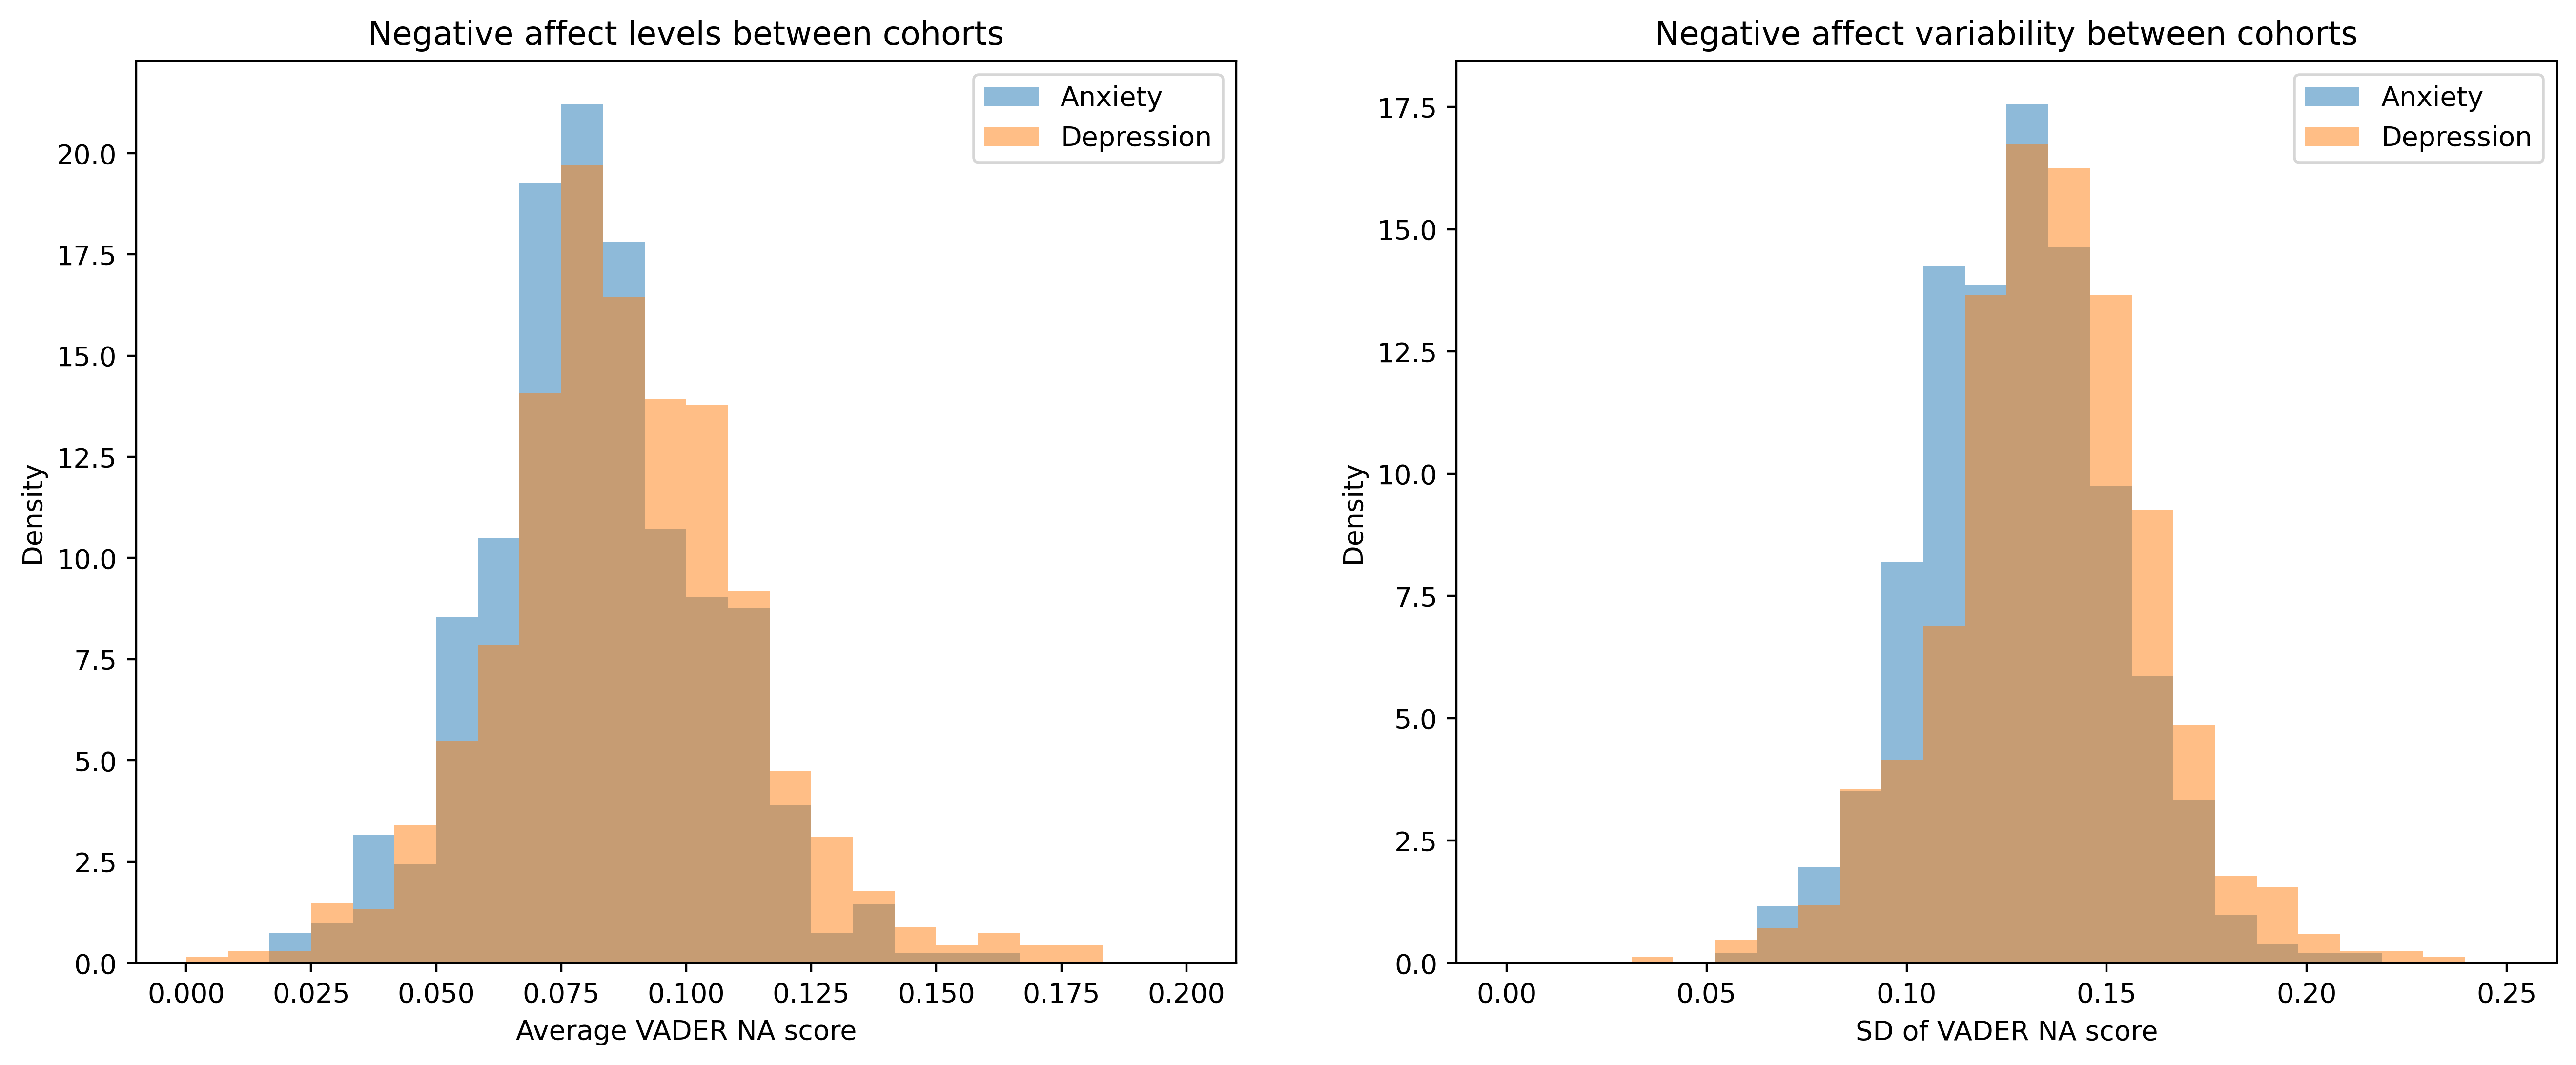
\includegraphics[width=\linewidth]{Images/na_histograms_overall.png}
    \caption{Negative affect level and spread across the entire time series, grouped by cohort.}
    \label{fig:overall_histograms}
\end{figure}

\subsubsection{6-hour windows}

%Moved to different section:
%Before interpreting the results obtained from the 6-hour window approach, it is crucial to assess whether the arithmetic mean and standard deviation serve as appropriate summary statistics for aggregating negative affect (NA) levels and their variability across individuals. If these measures fail to accurately represent the underlying distributions, subsequent inferences may be biased or misleading.

%To evaluate this assumption, the distributions of aggregated values for each subject are examined by comparing their means and medians. A significant difference between these measures would suggest that the data is skewed or contains outliers, potentially violating the assumption that the arithmetic mean is a robust central tendency measure. In the case of negative affect levels, computed as the mean across all 6-hour windows per subject, this assumption does not hold ($U = 1820498$, $p < .001$), indicating that the mean may not adequately summarize the distribution of NA levels.

%A similar issue is observed for negative affect variability, measured as the standard deviation across all 6-hour windows per subject. The significant test result ($U = 2187117.5$, $p < .001$) suggests that the standard deviation may not be the most reliable measure of variability, which requires careful interpretation of subsequent analyses.

\begin{figure}[h]
    \centering
    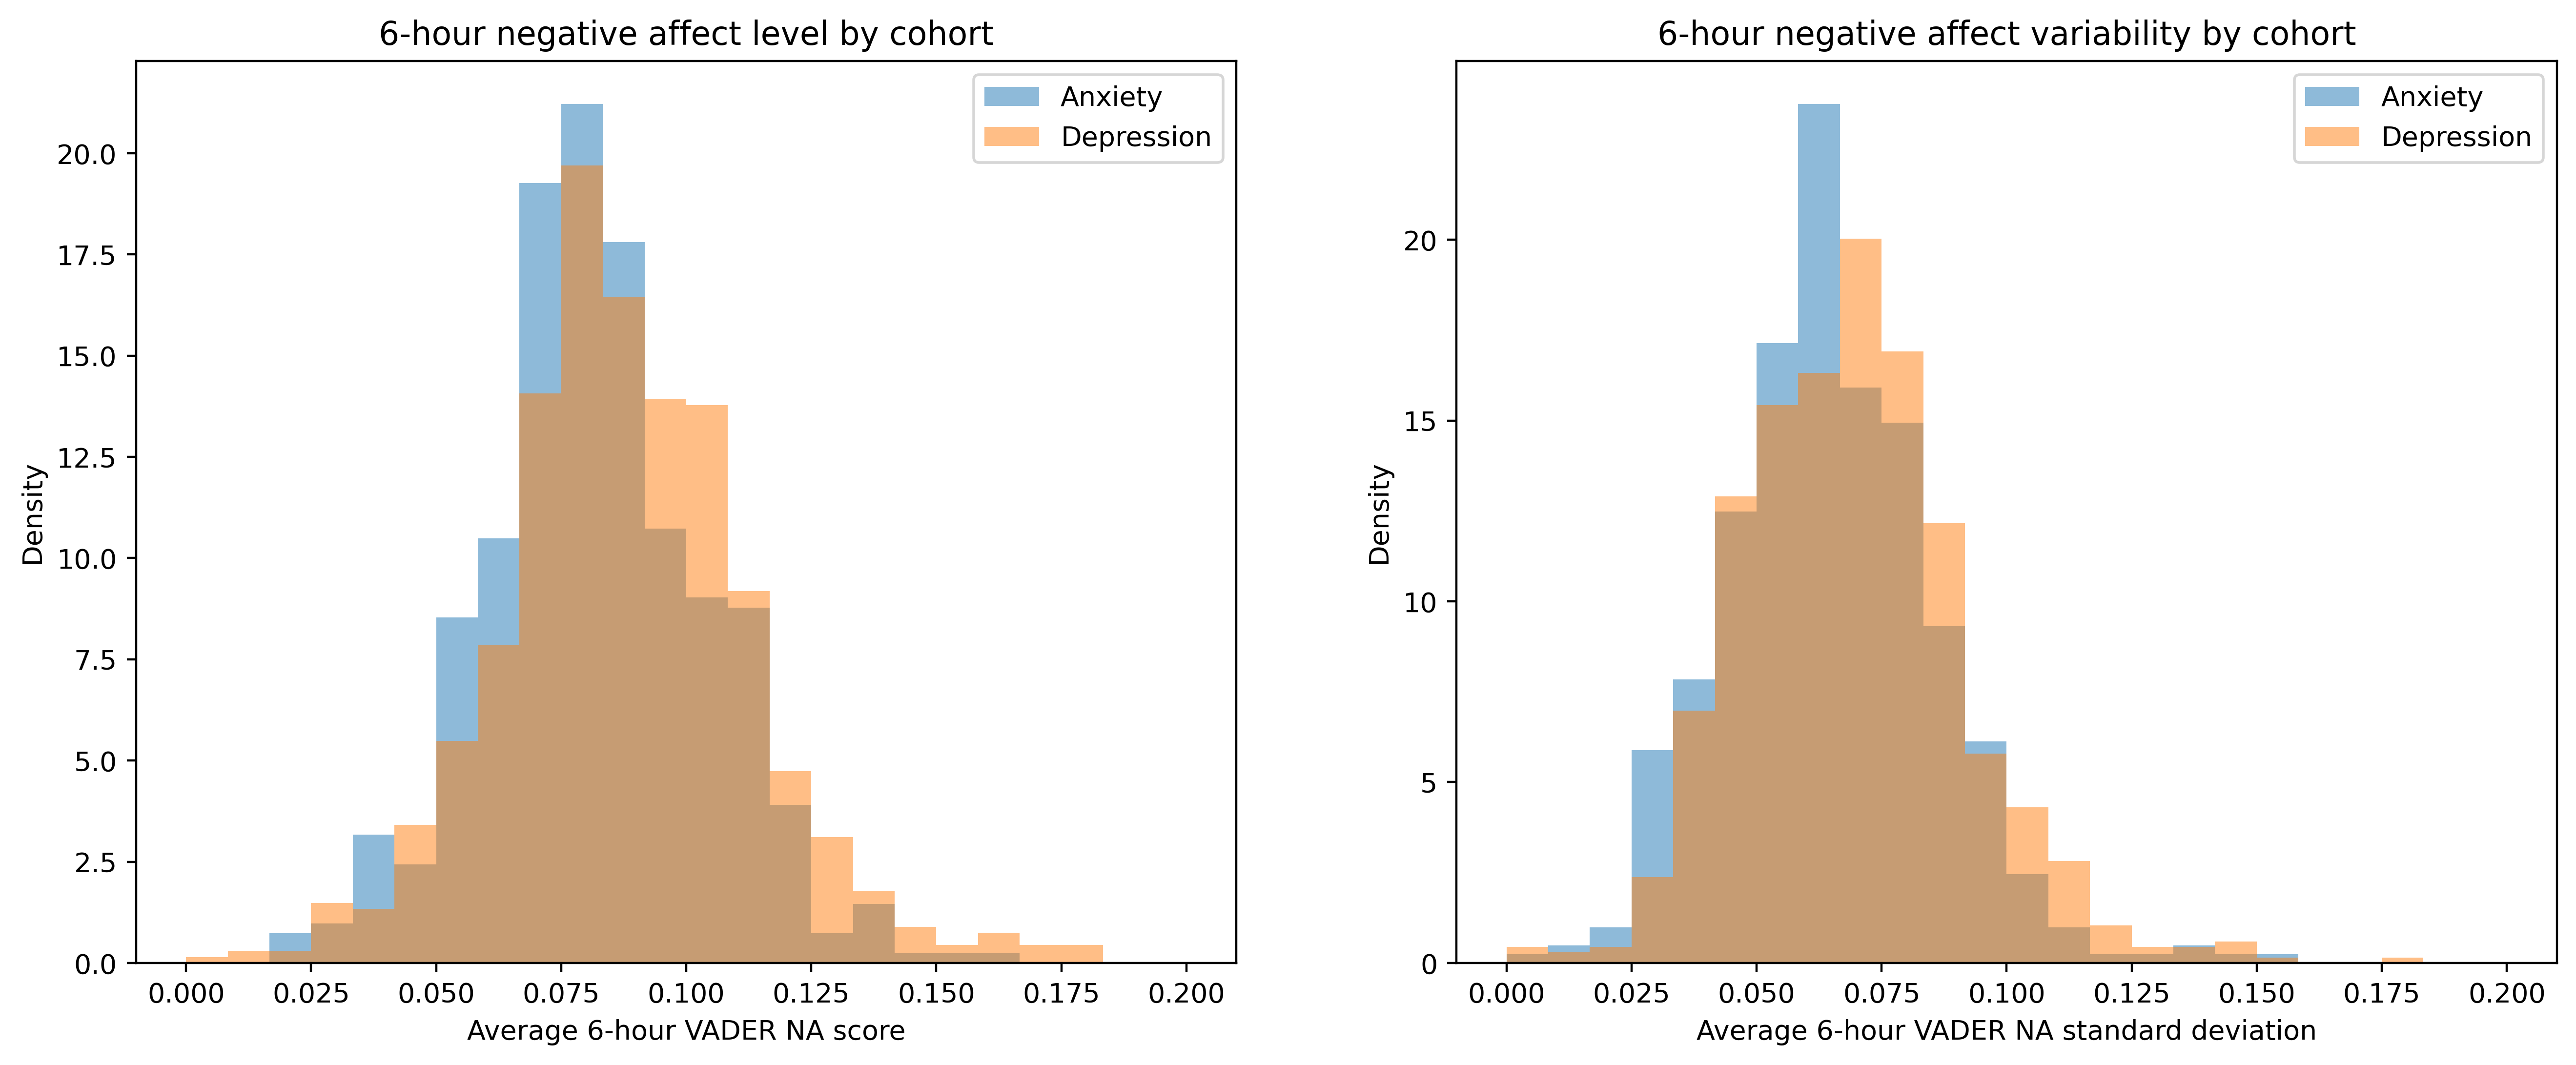
\includegraphics[width=\linewidth]{Images/na_histograms_6hr.png}
    \caption{Negative affect level and spread during 6-hour windows, grouped by cohort.}
    \label{fig:6hr_histograms}
\end{figure}

Figure \ref{fig:6hr_histograms} presents the distributions of negative affect levels and variabilities across subjects. Consistent with previous findings, the depression cohort had significantly higher NA levels than the anxiety cohort. Specifically, the mean NA level for the depression cohort was 0.0881, compared to 0.0823 in the anxiety cohort ($U = 636510$, $p < .001$). This result reinforces the distinction between the two clinical groups, with individuals diagnosed with depression expressing more pronounced negative affect.

Beyond differences in absolute NA levels, the depression cohort also demonstrated significantly greater variability in negative affect, with a mean variability of 0.0693 compared to 0.0648 in the anxiety cohort ($U = 1050891$, $p < .001$). This finding suggests that individuals with depression not only experience heightened negative affect but also exhibit more unstable affective patterns over time.

\subsubsection{Daily aggregation}

With each person's daily NA level fluctuations reduced to a single average value, the distributions as shown in Figure~\ref{fig:daily_histograms} emerged. Again, the depression cohort showed significantly higher NA levels than the anxiety cohort. Specifically, the mean NA level for the depression cohort was $0.0873$, compared to $0.0822$ in the anxiety cohort ($U = 222435$, $p < .001$). This result agrees with the previous finding.

Furthermore, the depression cohort exhibited significantly greater variability in negative affect, with a mean variability of $0.0885$ compared to $0.0809$ in the anxiety cohort ($U = 224679$, $p < .001$). This also supports the results from the 6-hour windows and indicates that NA variability is lower for the A cohort than the D cohort, supporting the hypothesized differences according to the CAM.

\begin{figure}[h]
    \centering
    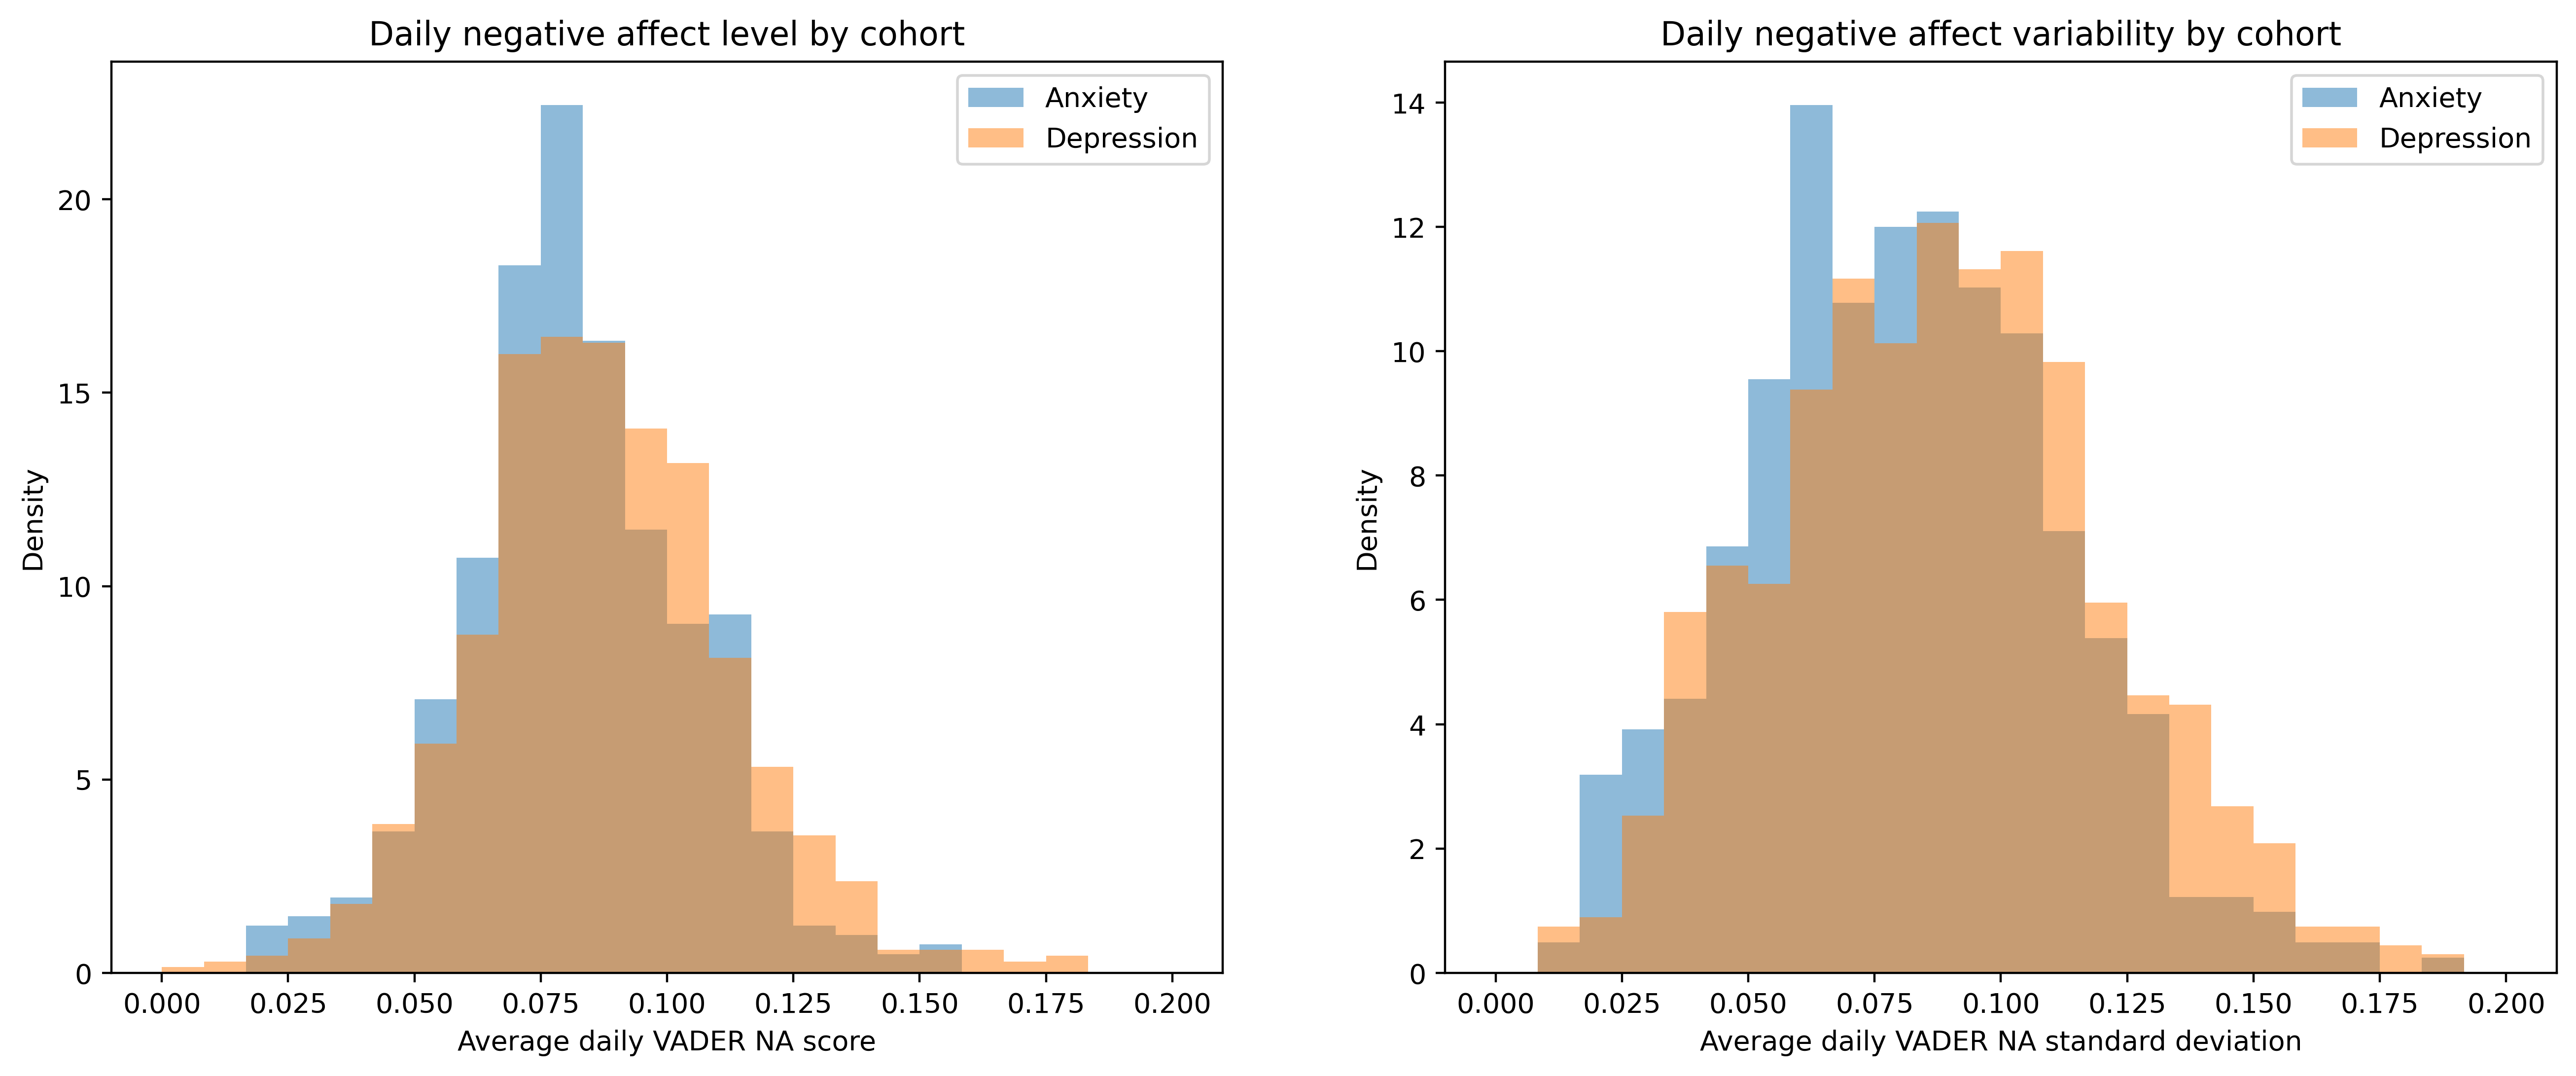
\includegraphics[width=\linewidth]{Images/na_histograms_daily.png}
    \caption{Negative affect level and spread during daily windows, grouped by cohort.}
    \label{fig:daily_histograms}
\end{figure}


\subsection{LMM}

In this section, the results for the linear mixed model approach are presented. First, results for tweet-level sentiments are shown, then for 6-hour aggregations.

\subsubsection{No aggregation}

Fitting the LMM to the whole dataset, the optimal spline knot placement according to RMSE was three knots with a polynomial degree of two, placed at 6 AM, 12 AM and 6 PM.

The spline plot, shown in Figure~\ref{fig:spline_preds_raw}, shows how NA levels were relatively stable throughout the day, with a pronounced peak in the afternoon, between 1 PM and 5 PM.

\begin{figure}[h]
    \centering
    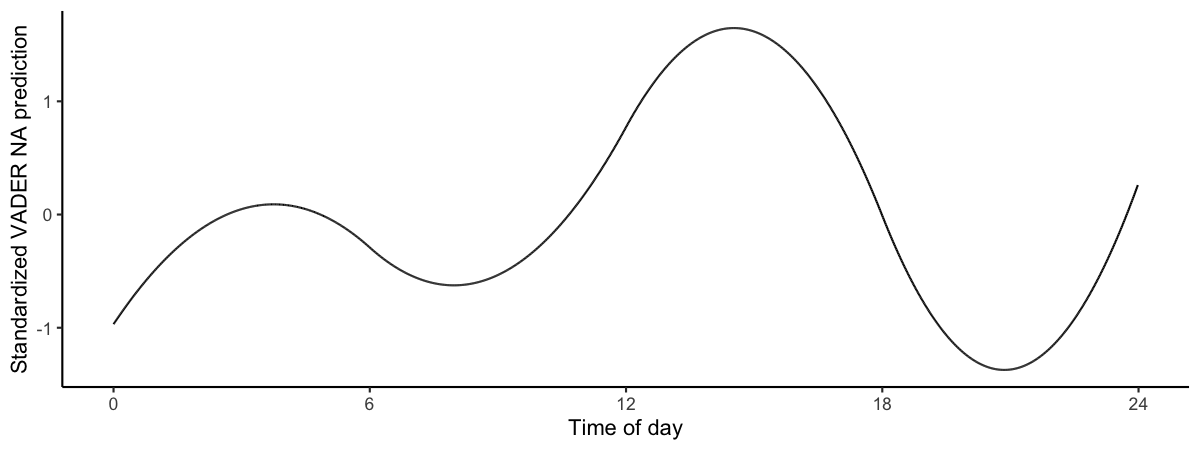
\includegraphics[width=\linewidth]{Images/lmm_raw_spline.png}
    \caption{Spline fit from LMM on tweet-level VADER-based sentiment data.}
    \label{fig:spline_preds_raw}
\end{figure}

The model represented a very weak fit, indicated by conditional $R^2$ of $0.03$. This was likely due to the large amount of single tweets and heterogeneous NA levels when not applying any smoothing function.

The model revealed a strong positive autocorrelation in the VADER NA scores, with a significant regression coefficient for the previous NA score ($B = 0.0488; p < .001$), suggesting that individuals' current NA levels are influenced by their previous NA levels, highlighting temporal dependence in emotional expression.

The time between consecutive tweets did not have a significant impact on NA scores ($B = -0.00005; p = .29$), indicating that the timing or duration between social media posts does not notably affect participants' NA levels, suggesting that posting frequency is not a strong predictor of emotional changes.

Although NA levels tended to be slightly higher on weekends, the difference was not statistically significant ($B = 0.0005; p = .08$), suggesting that the observed weekend effect on NA levels may be due to random variation rather than a consistent pattern.

However, NA variability was significantly greater on weekends compared to weekdays ($F(1, 1130402) = 12.703; p < .001$), with a standard deviation of $0.136$ on weekends versus $0.135$ on weekdays. This indicates that, while NA levels themselves may not differ, there is greater fluctuation in emotional experiences over the weekend, possibly reflecting changes in mood or social interaction patterns.

No significant differences were found across age groups in NA levels, suggesting that age does not significantly impact the average level of negative affect experienced by participants in this study.

Additionally, there were no significant gender differences in NA levels ($B = 0.0007; p = .62$), indicating that men and women in this sample report similar average levels of negative affect, despite potential differences in emotional experiences or expression.

Women showed significantly lower NA variability ($F(1, 1130402) = 7.17; p = .007$), with a residual standard deviation of $0.134$, compared to $0.136$ for men. This suggests that women may experience more stable emotional states, with less fluctuation in their NA levels across time.

Participants in the A cohort exhibited significantly lower NA levels than participants in the D cohort ($B = -0.0054; p < .001$), indicating that individuals with anxiety generally report lower negative affect compared to those with depression, consistent with the clinical distinction between the two conditions.

\begin{figure}
    \centering
    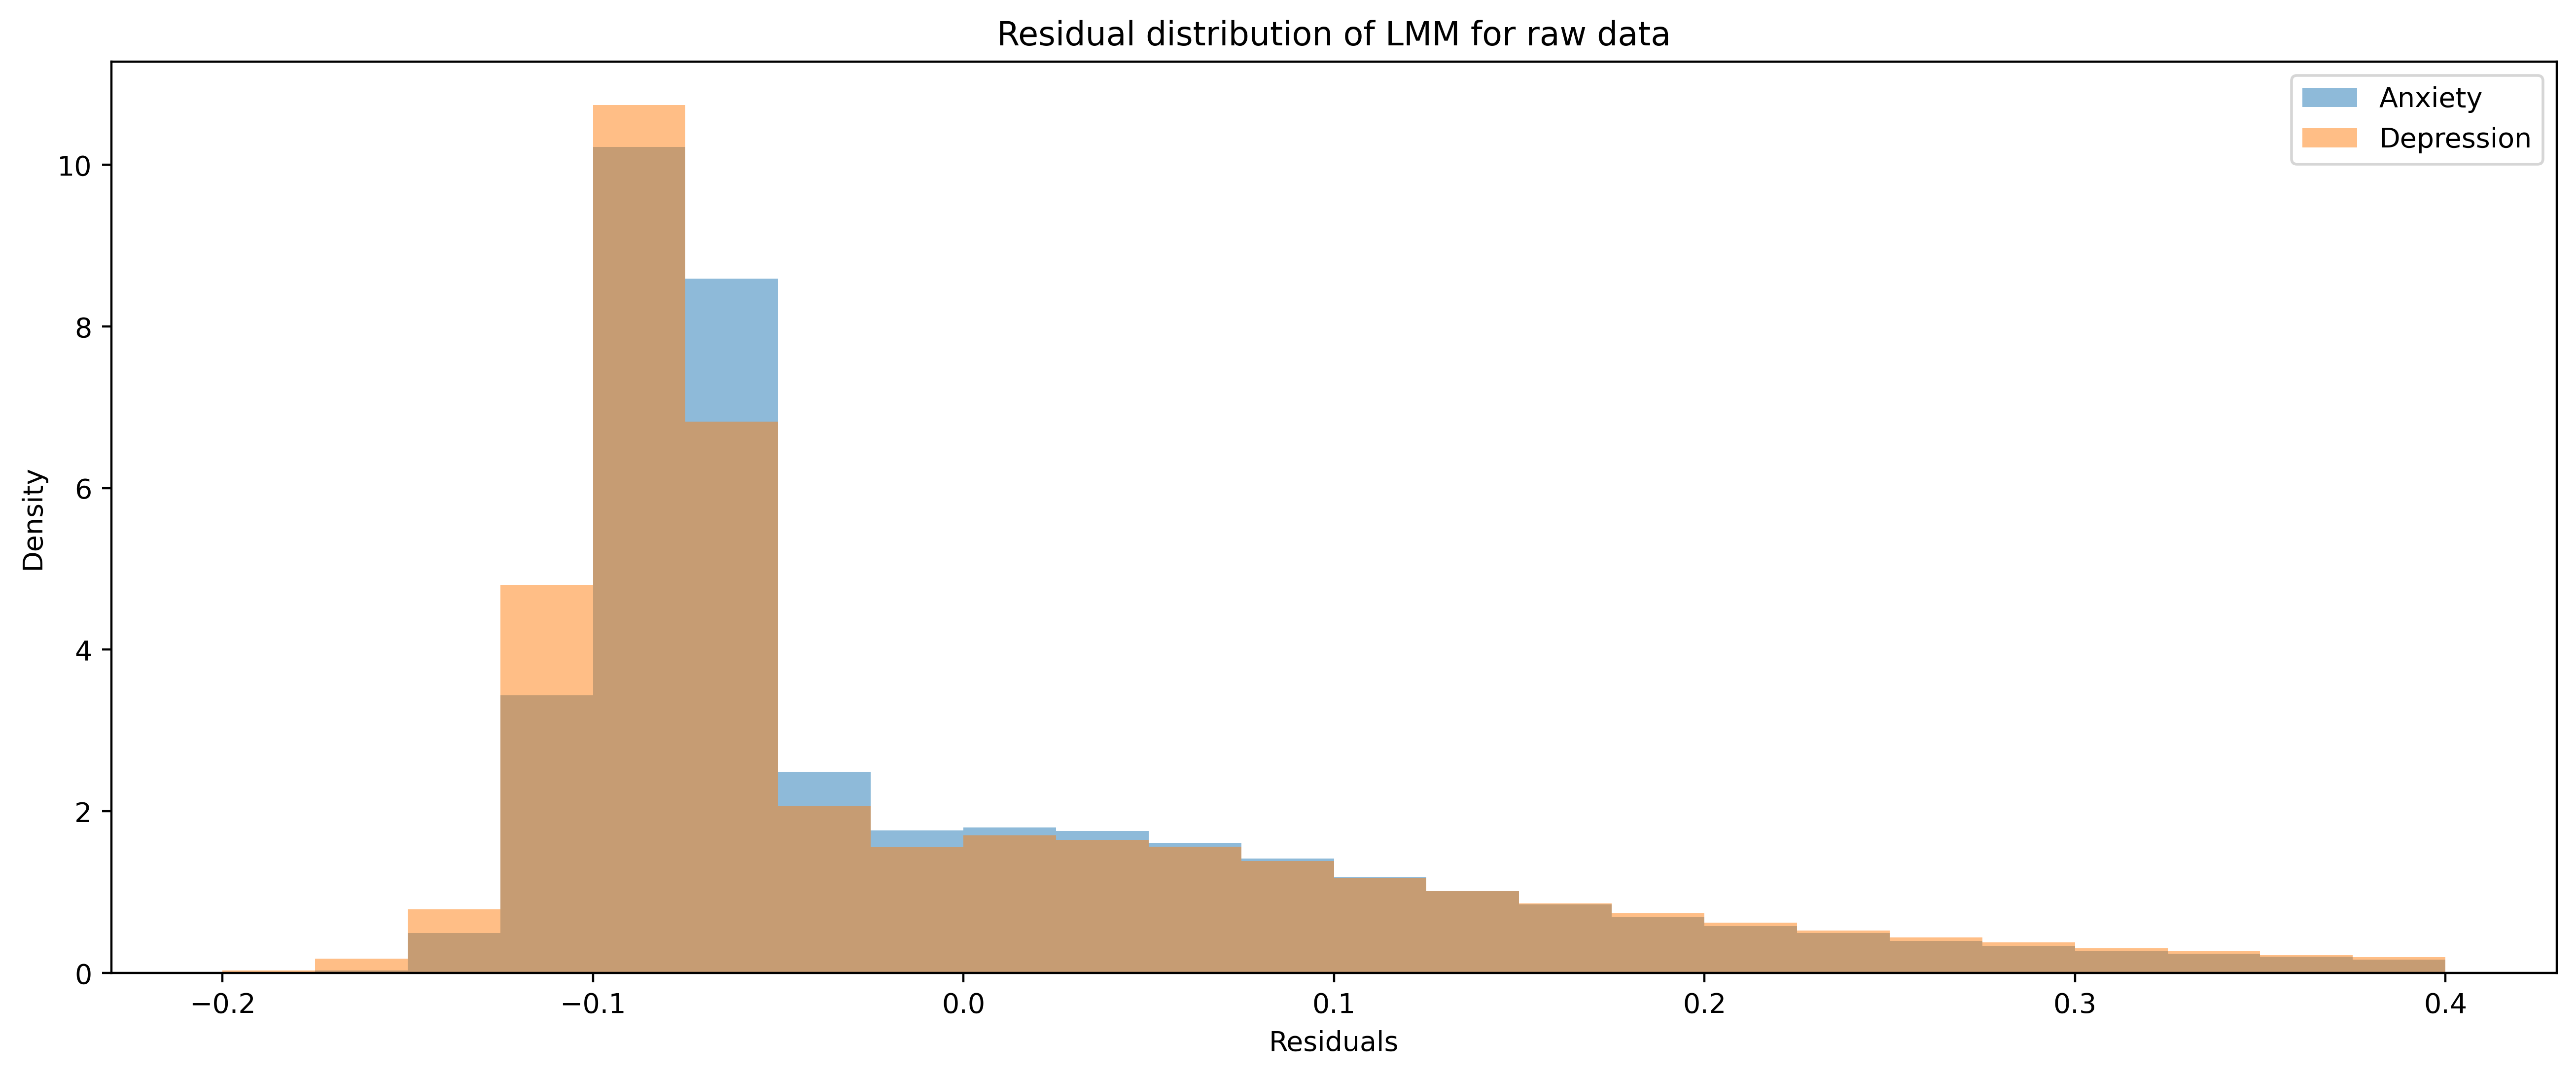
\includegraphics[width=\linewidth]{Images/lmm_raw_vader_residuals.png}
    \caption{Residual distribution by cohort for raw data LMM predictions}
    \label{fig:raw_lmm_hist}
\end{figure}

Furthermore, the A cohort showed lower NA variability (see Figure~\ref{fig:raw_lmm_hist}), with a residual standard deviation of $0.130$, compared to $0.138$ in the D cohort. This difference in variability was highly significant ($F(1, 1130402) = 713.84; p < .001$), suggesting that depression patients experience greater fluctuations in negative affect, potentially reflecting the emotional instability often associated with depressive disorders.

\subsubsection{6-hour windows}

Using 6-hour aggregated data, the optimal placement of spline knots was determined to be four equidistant knots placed throughout the day, with a polynomial degree of three. This configuration provided a balance between flexibility and parsimony, allowing the model to capture meaningful fluctuations in NA levels without overfitting to short-term variations.

The resulting spline fit is illustrated in Figure \ref{fig:spline_preds_6hr}. The fitted curve reveals a distinct increase in NA levels around 4 AM, suggesting an increase in engagement with emotionally negative content during the early morning hours. Following this rise, NA levels remain relatively stable throughout the rest of the day, with no pronounced peaks or troughs.

\begin{figure}[h]
    \centering
    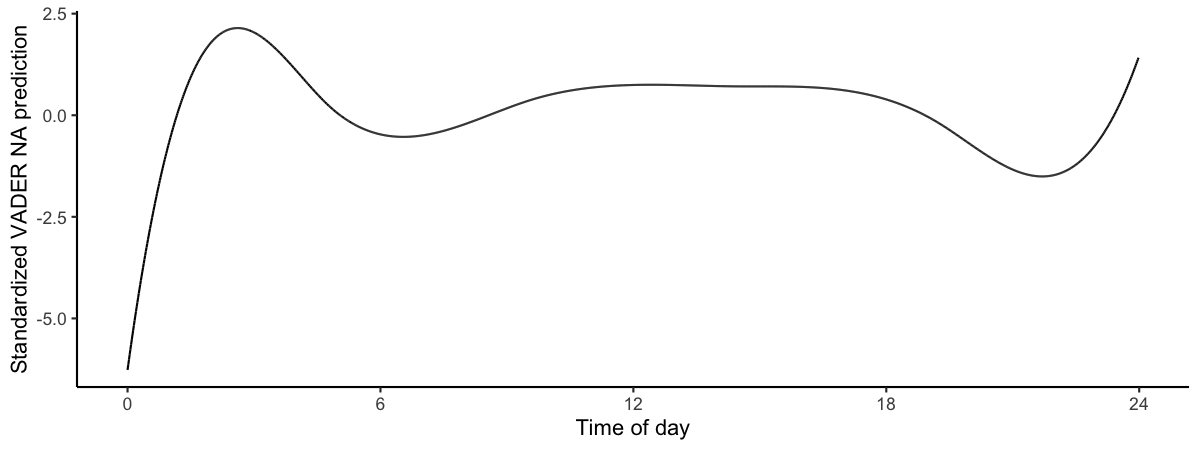
\includegraphics[width=\linewidth]{Images/lmm_6hr_spline.png}
    \caption{Spline fit from LMM on 6-hour windowed VADER-based sentiment data.}
    \label{fig:spline_preds_6hr}
\end{figure}

The model demonstrated a good fit, with an explained variance of $R^2 = 0.51$ as measured by conditional $R^2$. While this suggests that a significant portion of the variance in NA levels can be accounted for by the predictors included, a substantial proportion remains unexplained, likely due to unmeasured individual differences or external contextual factors.

The previous (autoregressive) VADER NA score exhibited a strong positive association with the current NA score ($b = 0.69$, $p < .001$), indicating that an individual's emotional state is highly correlated across consecutive tweets. This suggests a degree of temporal stability in NA levels, wherein prior emotional states strongly influence subsequent affective expression.

In contrast, the time elapsed between tweets did not show a statistically significant relationship with NA levels ($b = -0.000004$, $p = .85$). This suggests that the passage of time alone is not a meaningful predictor of fluctuations in expressed negative affect, at least within the timeframes typically observed in social media activity.

Tweets posted on weekends differed significantly in NA levels compared to those posted on weekdays ($b = 0.0002$, $p = .23$). This indicates that, on average, individuals express lower levels of negative affect throughout the week, with notable fluctuations between workdays and leisure days. In addition to the mean levels, an important difference also emerges when considering the variability in NA scores.

Residual variance, as a measure of NA variability, differed significantly between weekday and weekend tweets ($F(1, 1116317) = 8.69$, $p = .003$). Specifically, tweets posted on weekdays exhibited greater residual variance, implying that NA expression becomes less predictable during these periods. This suggests that individuals may experience more erratic emotional states on weekdays, potentially due to less focus on social and personal experiences.

None of the categorical age features had a significant association with NA levels, indicating that there are no systematic differences in expressed negative affect across age groups. This suggests that, at least within the sampled population, age does not meaningfully influence the extent of negative emotional expression on social media.

Similarly, no significant difference in NA levels was observed between men and women ($b = 0.0002$, $p = .68$). This finding aligns with previous research suggesting that while gender differences exist in broader emotional regulation and coping strategies, they may not necessarily manifest in overall levels of expressed negative affect.

However, while mean NA levels did not differ between genders, the variability in NA levels was different for men than for women. Levene's test for homogeneity of variance revealed significantly higher residual variance for women ($F(1, 1116317) = 44.56$, $p < .001$), indicating greater fluctuations in negative affect over time. This suggests that while men and women may express similar levels of negative affect on average, women's affective states appear to be more dynamic and less stable over time.

Membership in the anxiety cohort was found to be negatively associated with NA levels ($b = -0.0017$, $p < .001$), suggesting that individuals diagnosed with anxiety tend to express lower levels of negative affect than those diagnosed with depression. This finding is consistent with prior research indicating that while both conditions involve dysregulated affect, depression is typically characterized by more persistent and severe negative emotional states.

Beyond differences in NA levels, the two cohorts also differed in the predictability of their negative affect expression. The residual variance for the anxiety cohort was $0.0472$, compared to $0.0480$ for the depression cohort. As shown in Figure \ref{fig:6hrlmm_cohort_hist}, this difference was statistically significant ($F(1, 1116317) = 67.59$, $p < .001$). These results indicate that individuals with depression not only experience higher average levels of NA but also exhibit greater fluctuations in their negative affective expression, making their emotional states less predictable compared to those in the anxiety cohort.



\begin{figure}[h]
    \centering
    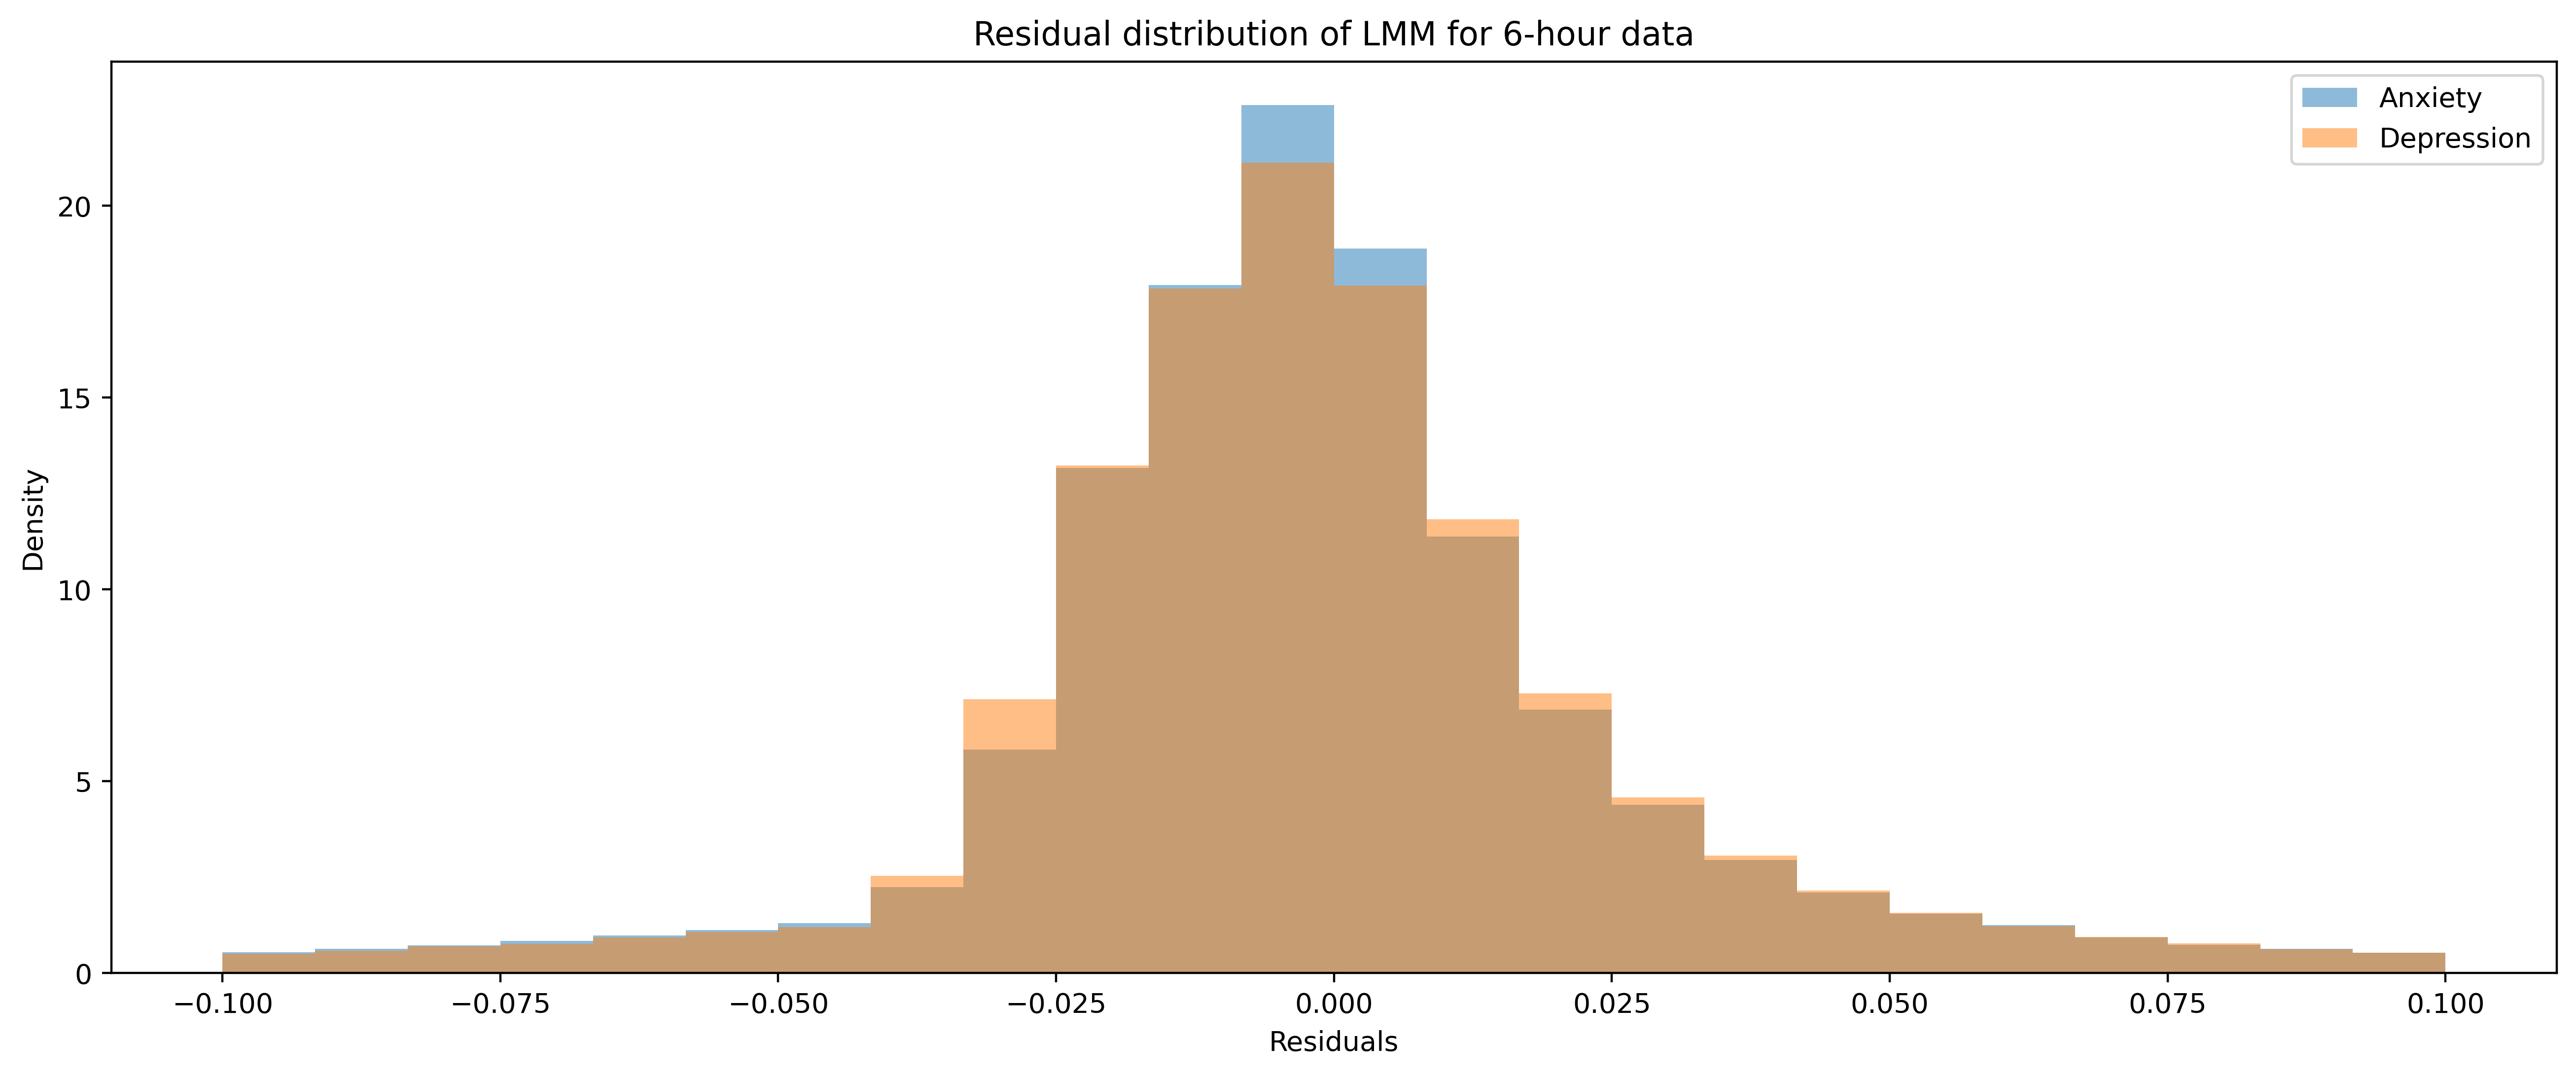
\includegraphics[width=\linewidth]{Images/lmm_6hr_vader_residuals.png}
    \caption{Residual distribution by cohort for 6-hour-windowed LMM predictions}
    \label{fig:6hrlmm_cohort_hist}
\end{figure}


\subsection{Robustness checks}

\subsubsection{Transformer-based analyses}

Prior to re-running the analyses based on RoBERTa-derived sentiment scores, the relationship between these scores and those obtained using the VADER approach was examined. Specifically, a Pearson correlation coefficient was calculated to assess the degree of linear association between the two sentiment measures across the full dataset. The resulting correlation coefficient was $r = 0.001$, indicating virtually no linear relationship between the VADER and RoBERTa sentiment scores. This lack of correlation suggests that the two methods capture fundamentally different aspects of sentiment within the data. Consequently, subsequent analyses based on RoBERTa scores may offer a distinct and potentially complementary perspective on the distribution of NA levels in the sample, independent of the VADER-based results.

As for the VADER-based analyses, the assumption of (approximate) symmetric NA level distributions was also checked for the RoBERTa scores. For the raw tweet-level data, the assumption did not hold since within-person mean and median are significantly different ($U = 167521; p < .001$). For the 6-hour windows, the assumption could not be rejected, since the means and medians of 6-hour window average scores for each person were not significantly different ($U = 113207; p = .07$). For daily aggregated data, again, the assumption did not hold ($U = 125065; p < .001$).

When applying the transformer-based sentiment analysis without any windowed aggregation — that is, based on raw, tweet-level sentiment estimates — significant differences in NA levels were observed between the A and D cohorts. Specifically, a Mann-Whitney U test indicated that NA levels differ significantly across groups ($U = 29385; p = .04$), with the average NA score being higher for the D cohort ($M = .2978$) compared to the A cohort ($M = .2792$). 

When examining NA variability, operationalized as the within-user standard deviation of NA scores, significant differences did not emerge between the two cohorts ($U = 27326; p = .58$). The D cohort again showed slightly higher average variability in NA ($M = .3196$) compared to the A cohort ($M = .3189$). Thus, the sample mean standard deviation was higher for the D cohort, although not statistically significant.

Similar results were found for the 6-hour aggregated data. The average NA level was higher in the D cohort with $.30$ compared to $.28$ for the A cohort ($U = 29364; p = .04$). There was no significant difference in NA variability though ($U = 26259; p = .89$). Descriptively, the A cohort showed slightly higher variability with a standard deviation of $.1789$ as compared to $.1786$ for the D cohort.

For daily aggregations, the D cohort again showed higher NA levels ($.29$) compared to the A cohort ($.27$), which was statistically significant ($U = 29318; p = .04$). The differences in NA variability were also not significant ($U = 26830; p = .79$), although the D cohort had slightly higher variability again ($.22$ compared to $.21$).

In addition to the overall differences, LMM was also fitted to the RoBERTa data.

The LMM showed substantial explanatory performance, with a conditional $R^2 = .59$. This indicates, that the model fit is quite good and the covariates in the model are able to explain a substantial amount of the variation in the RoBERTa NA scores.

The splines knots were optimally placed at 6AM, 12 AM and 6 PM, with a polynomial degree of two. The spline fit can be seen in Figure \ref{fig:roberta-spline}. NA levels were highest during the morning (6-12 AM) and appeared to be otherwise relatively stable throughout the day.

\begin{figure}[h]
    \centering
    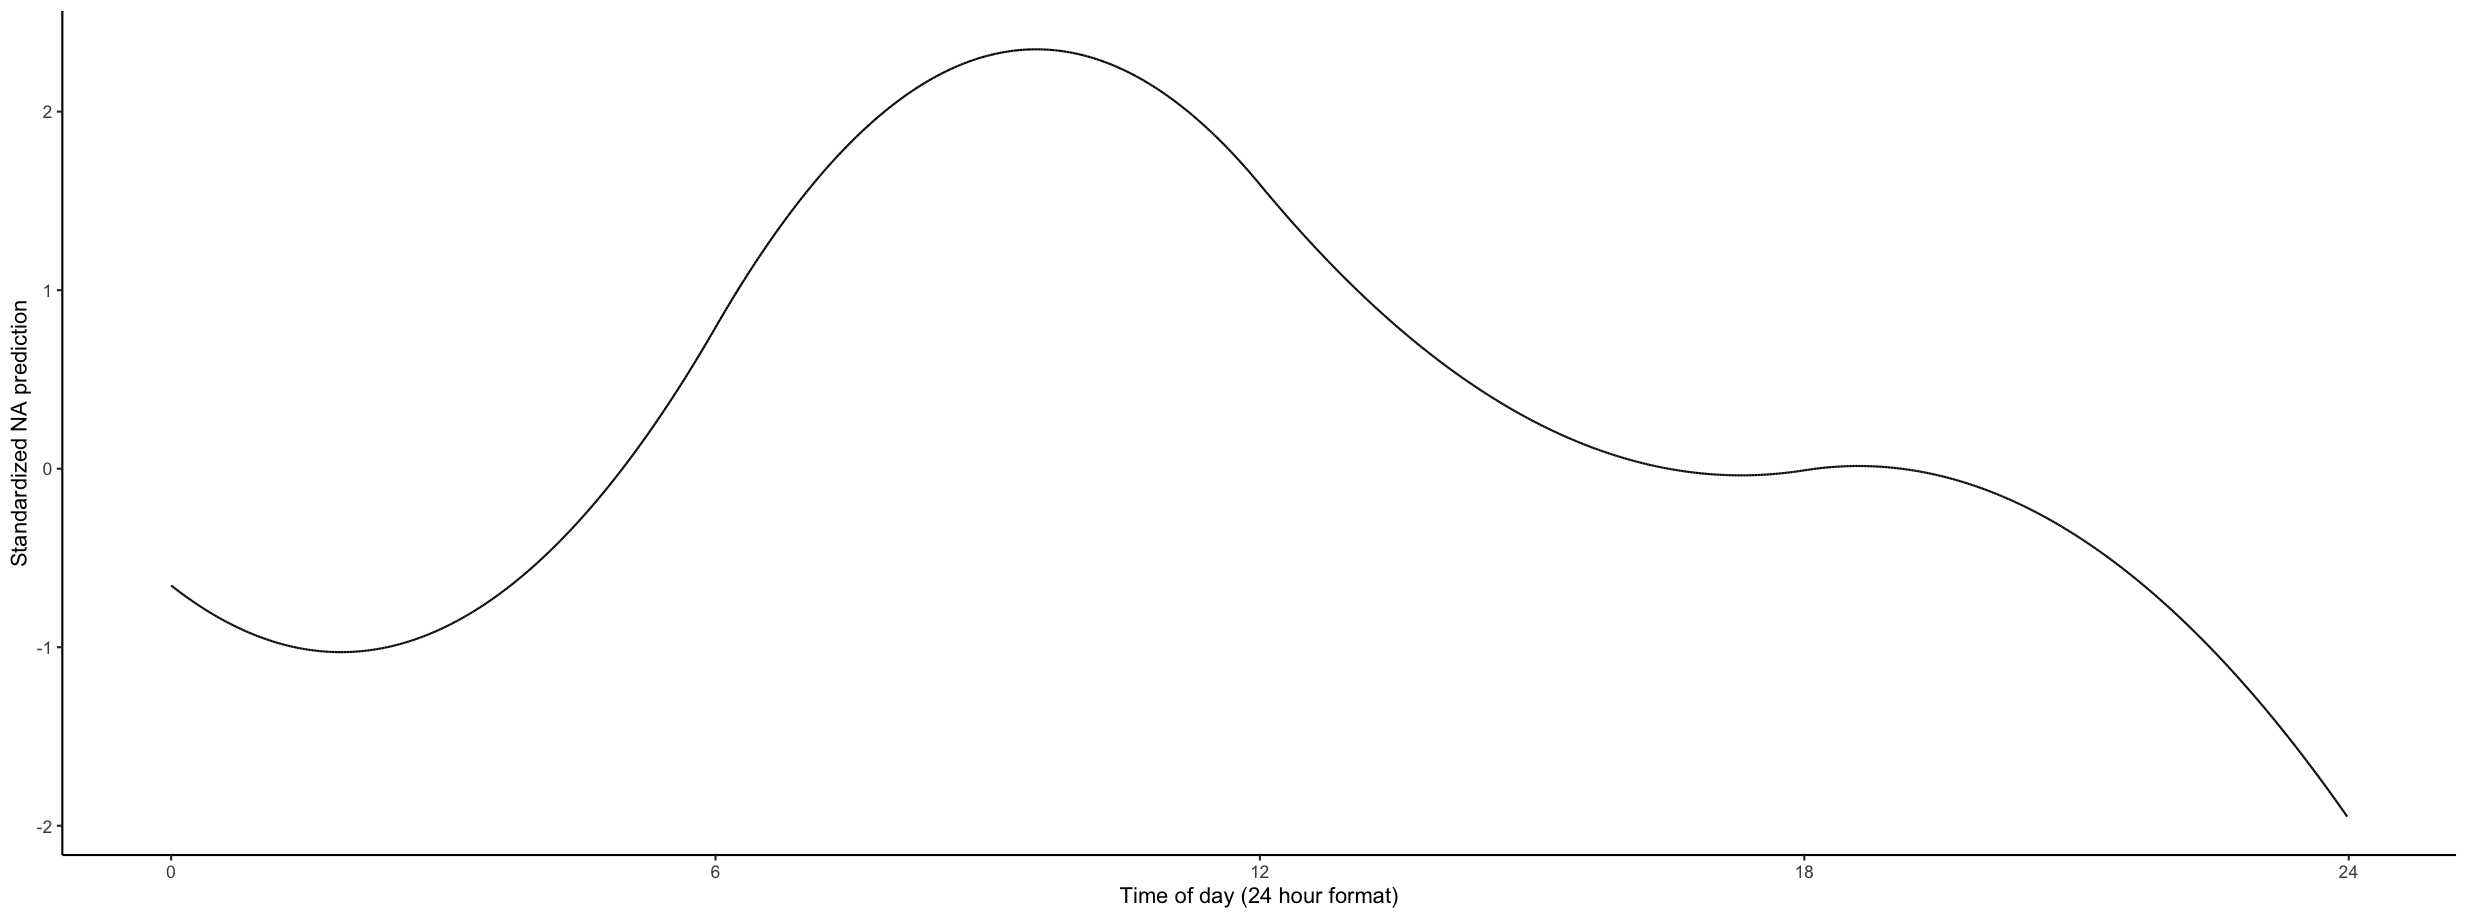
\includegraphics[width=\linewidth]{Images/roberta_lmm_splines.png}
    \caption{Spline fit from LMM on RoBERTa-based sentiment data of 250 sample participants.}
    \label{fig:roberta-spline}
\end{figure}

There was no difference between the genders regarding NA levels ($B = 0.0023; p = .45$) or the NA variability ($F(1, 279790) = 0.00; p = .99)$. Strong autocorrelation could still be observed between consecutive tweets ($B = 0.71; p < .001$). This indicates, that the baseline NA level for a 6-hour period is always offset by roughly $71\%$ of the NA level of the previous period.

NA levels were significantly lower on week ends ($B = -0.0009; p = .04$), indicating that users show less negative emotion online during the week ends.

%In the RoBERTa-based LMM, a statistically significant effect of the logarithmic time passed since the previous tweet could be observed ($B = -0.0012; p < .001$), indicating that NA levels tend to decrease over time when not actively posting on Twitter. More specifically, the point estimate suggests, that NA levels decline by $0.0012$ when multiplying the expired time by $e \approx 2.718$.

Using the RoBERTa NA scores as outcome variable, the anxiety cohort exhibited a higher NA variability as measured by residual standard deviation ($\sigma^2_A  = 0.123$) than the D cohort ($\sigma^2_D = 0.121$). This difference is statistically significant ($F(1, 407101) = 10.59; p = .001$). In order to further underline this finding, a nonparametric bootstrap procedure was run to compute confidence intervals for the difference in variability between the cohorts. In 1000 bootstrap replications, the 95 \% CI for the difference in variances is $[0.0007,  0.0030]$, further underlining, that the anxiety cohort showed higher residual variance and therefore higher NA variability. See Figure~\ref{fig:roberta-lmm-residuals} for a graphical representation of the residual distribution.

\begin{figure}
    \centering
    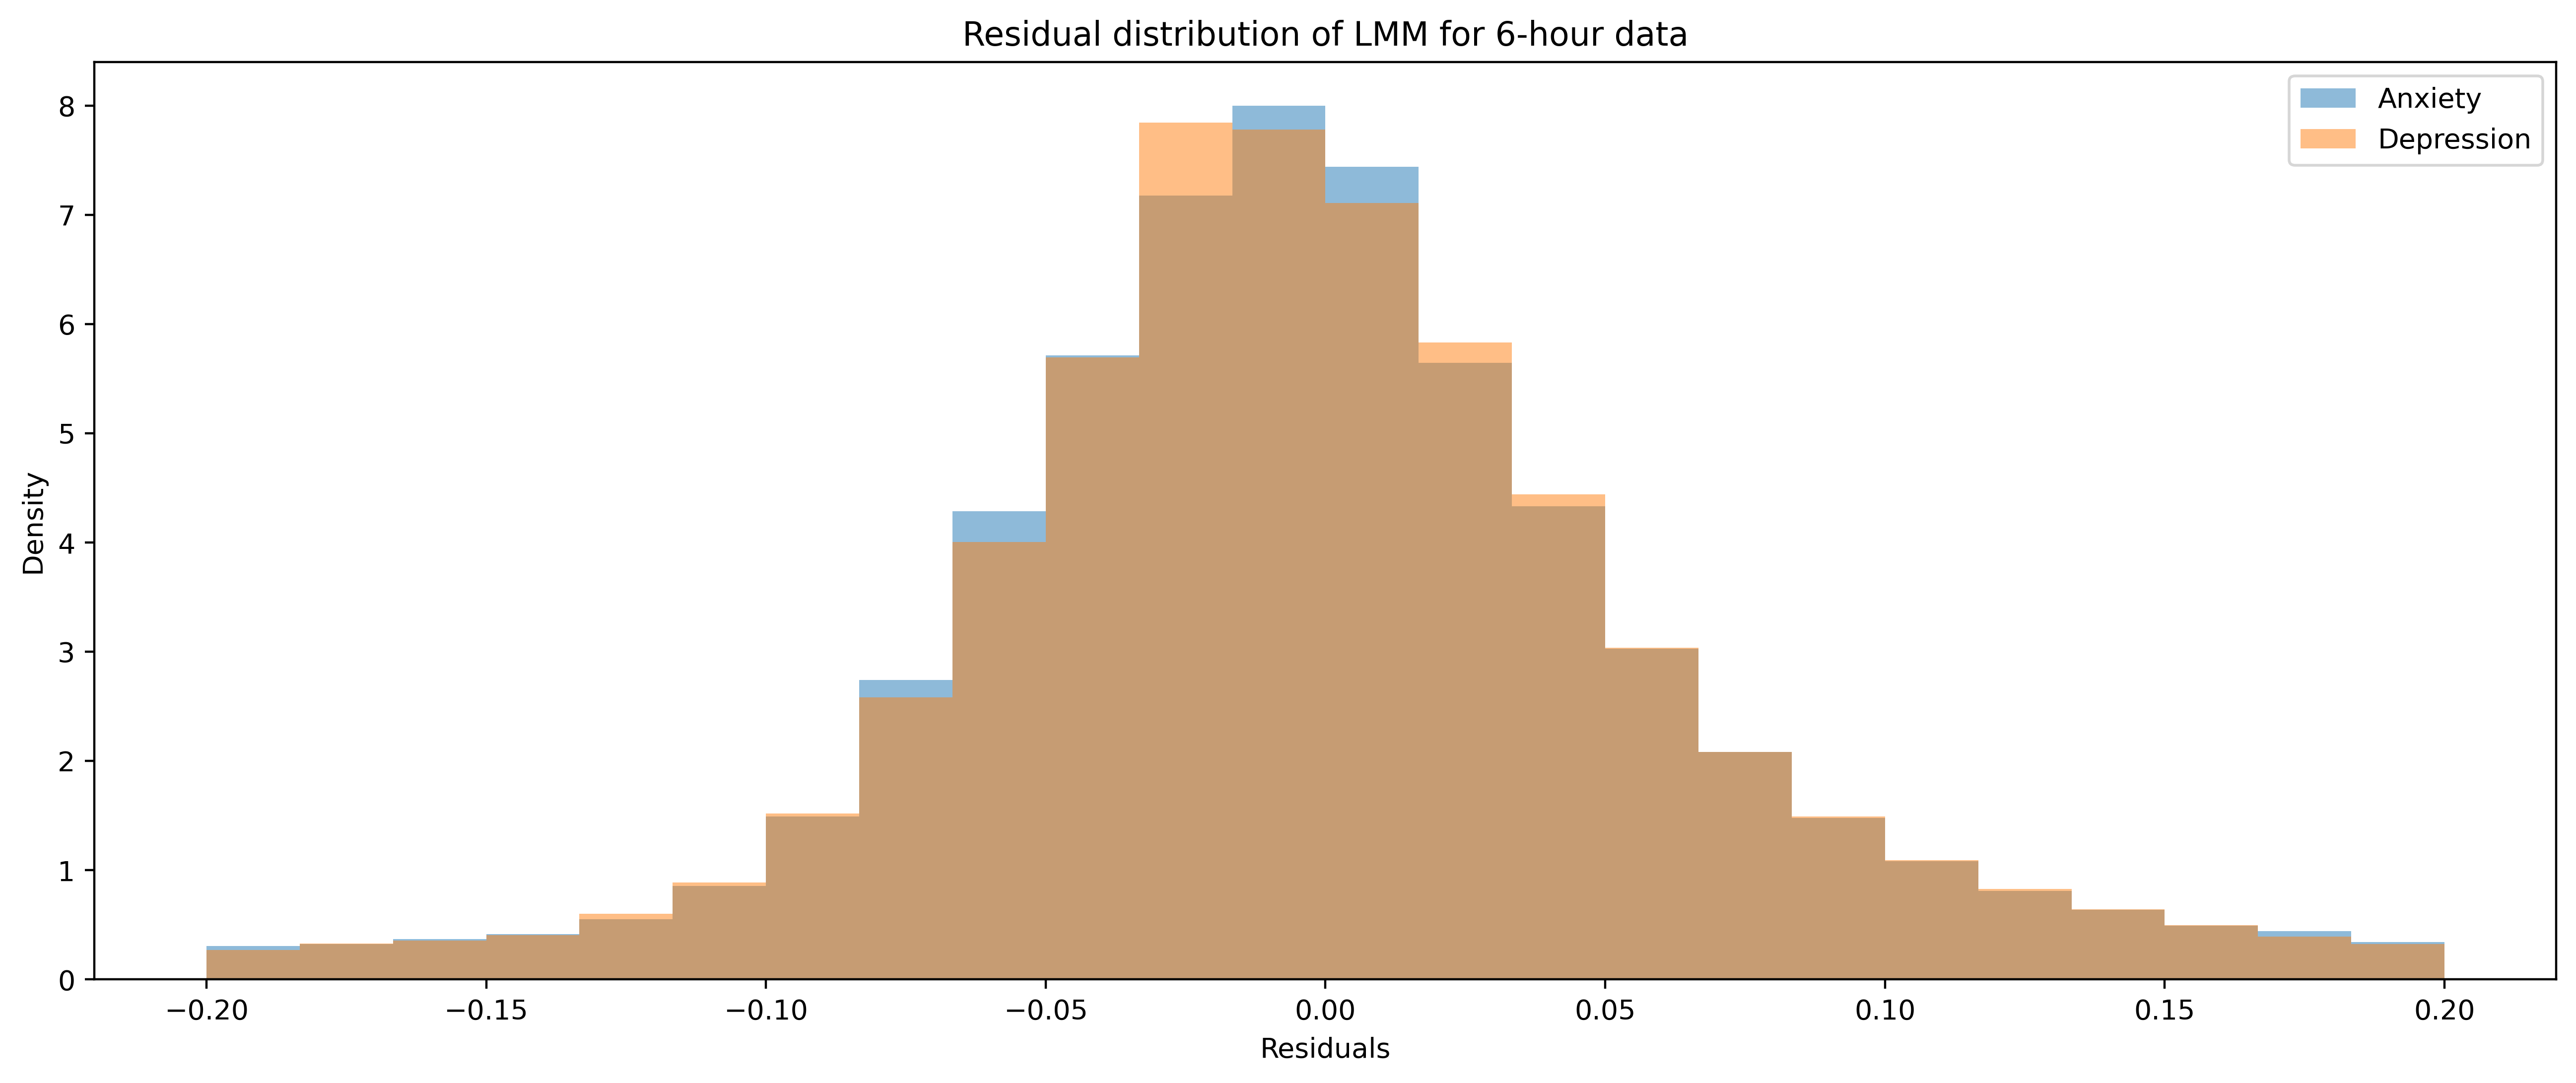
\includegraphics[width=\linewidth]{Images/lmm_6hr_roberta_residuals.png}
    \caption{Residual distribution for LMM predictions of 6-hour windowed RoBERTa NA scores.}
    \label{fig:roberta-lmm-residuals}
\end{figure}

The overall NA level was still significantly lower for the A cohort ($B = -0.0059; p = .04$), supporting earlier findings.

%TBD: This is counter-intuitive, but 
%it might be that our covariates dont fit anxiety patients
%otherwise interesting finding that anxiety patients appear to have higher NA variability
%future work: re-run the roberta analysis with all tweets

%Taken together, these findings suggest that — in the absence of temporal aggregation or smoothing — the transformer-based sentiment analysis does not capture statistically robust differences in either NA levels or NA variability between anxiety and depression groups, despite small descriptive differences pointing in the expected direction (see Figure \ref{fig:roberta_na_dist}. This further underscores the potential importance of modeling approach when attempting to extract NA information from online user activity data.



\begin{figure}[h]
    \centering
    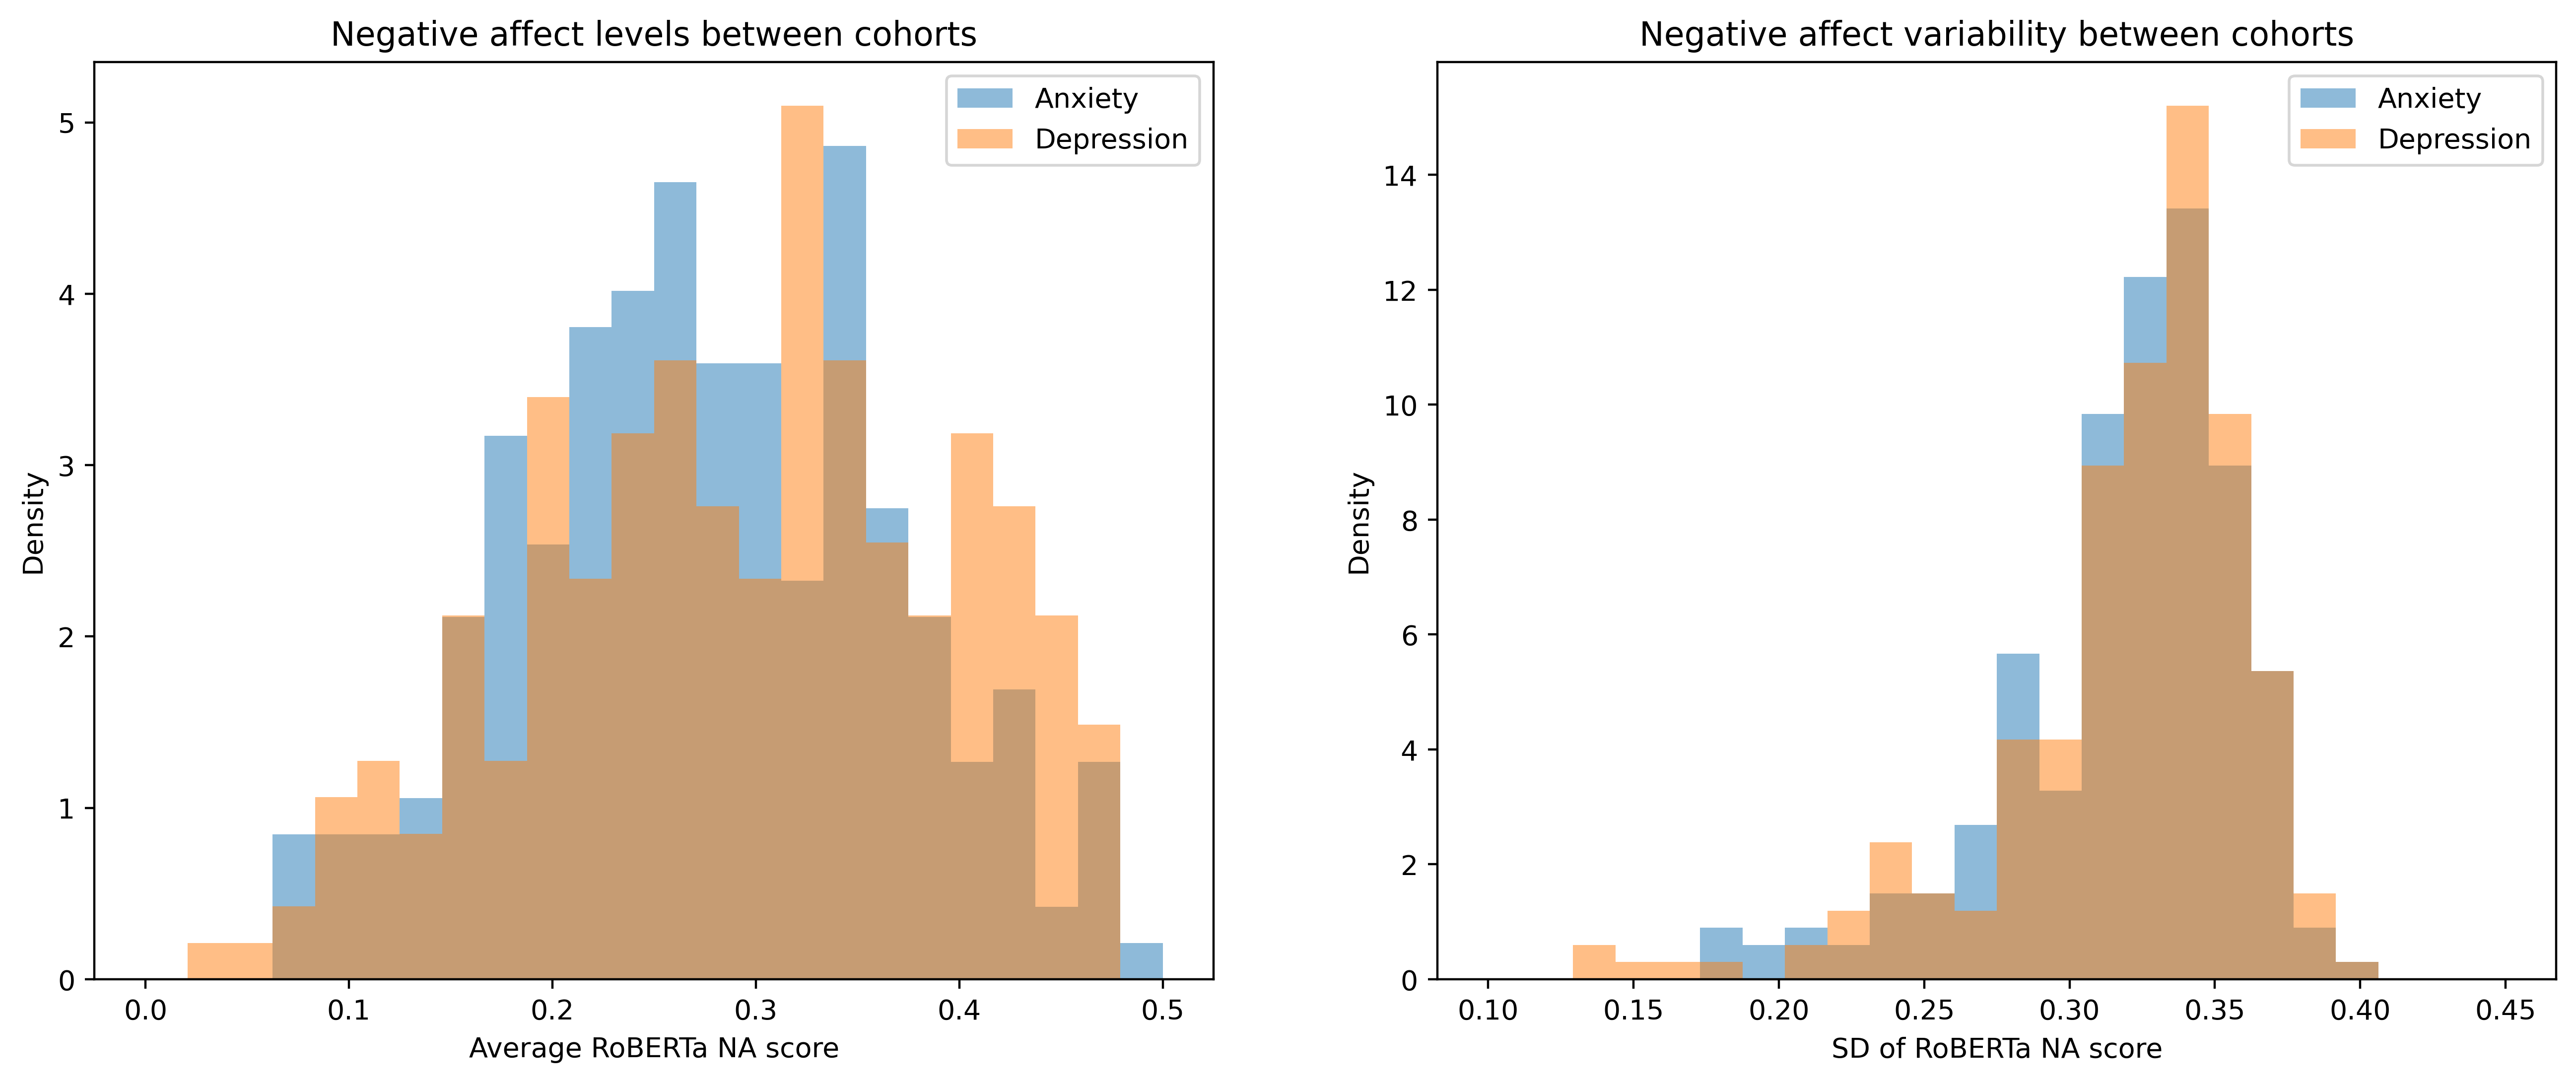
\includegraphics[width=\linewidth]{Images/na_histograms_raw_roberta.png}
    \caption{Means and standard deviations of RoBERTa NA scores across the entire time series.}
    \label{fig:roberta_na_dist}
\end{figure}



\subsubsection{Bounded distributions}

The paired sub-samples of the D and A cohorts showed to have highly similar mean VADER NA scores across the time series ($\bar{x}_D = 0.084883, \bar{x}_A = 0.084881$). The D cohort had a larger standard deviation with $\sigma^2_D = 0.134322$, while the A cohort had $\sigma^2_A = 0.130531$ (see Figure \ref{fig:bounded_boxes}).

This difference in standard deviation was statistically significant as shown by paired t-test ($t(647) = 4.86; p < .001$), indicating that the A cohort showed significantly lower NA variability than the D cohort, even when controlling for differences in overall NA levels.

\begin{figure}[h]
    \centering
    
\includegraphics[width=\linewidth]{Images/boxplot_depression_anxiety.png}
    \caption{Standard deviation and mean VADER NA score of paired sub-samples.}
    \label{fig:bounded_boxes}
\end{figure}

For the same analysis, but based on the RoBERTa sentiment estimations, a significant difference in NA variability between the cohorts also emerged. In this, case, it pointed to the opposite direction though. The A cohort had a larger standard deviation at $\sigma^2_A = 0.3248$, as opposed to $\sigma^2_D = 0.3215$ for the D cohort. The result was statistically significant ($t(183) = -2.19; p = .03$).

Thus, this indicates that anxiety patients actually showed higher NA variability than depression patients when comparing RoBERTa scores.


\begin{figure}[h]
    \centering
    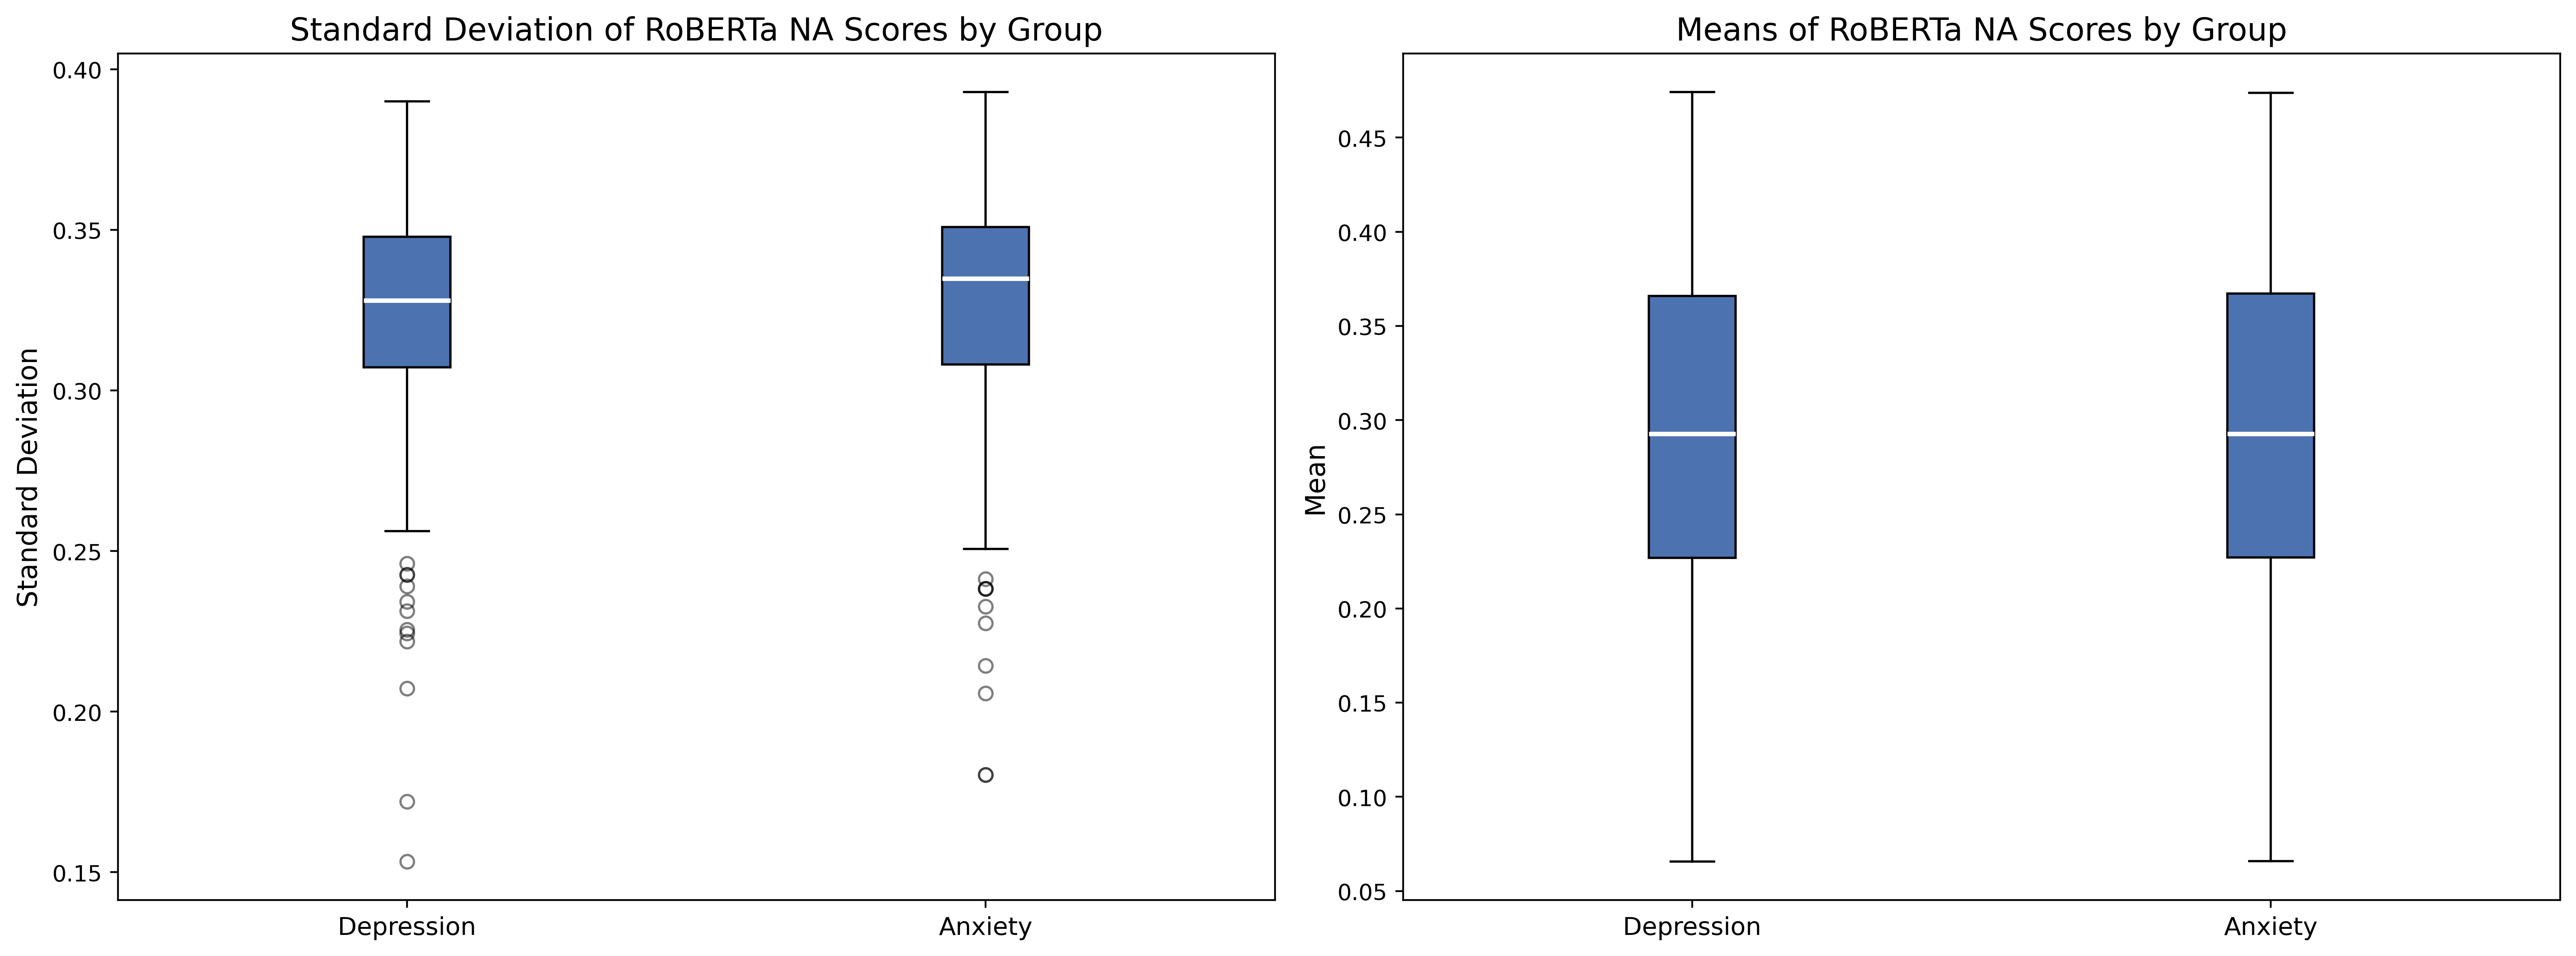
\includegraphics[width=\linewidth]{Images/boxplot_depression_anxiety_roberta.png}
    \caption{Standard deviation and mean RoBERTa NA score of paired sub-samples.}
    \label{fig:bounded_boxes}
\end{figure}

%\subsubsection{Notes...}
%- LMM
%    - If the previous tweet was more than an hour ago, it becomes much more %difficult to predict NA level
%    - results also remain for just checking tweets that had another recently
%- LMM based sentiments


\section{Conclusion}
\label{sec:conclusions}
%recap of results

The present study aimed at reproducing and improving upon the results from \citet{rutter2024}. They showed in their analysis, that twitter sentiment data could be used to empirically validate the CAM and the differences it proposed between anxiety and depression patients regarding their willingness to be exposed to fluctuation in NA levels. According to the CAM, anxiety patients are motivated to maintain a stable NA level in order to not be subjected to strong emotional shifts. This should be also visible in sentiments of published tweets, as measured by variability of NA level estimates.

Using the proposed method of \citet{rutter2024}, the findings could be exactly reproduced using simple mean and standard deviation comparisons between the cohorts. Depression patients showed significantly higher NA levels and NA variability than anxiety patients.

The same conclusions were reached using 6-hour windows, where tweet sentiments within 6-hour windows were aggregated. Here, again, depression patients showed higher NA levels and variability. A key methodological contribution of the present study lies in the extension of prior research through the introduction of windowed aggregation of sentiment data across time. While previous studies in this area have typically relied on aggregated sentiment scores computed across users' entire available time series, our approach applied moving windows to calculate NA levels and NA variability within smaller, temporally localized segments of user activity.

Thus, the previous findings were successfully replicated using these methods, indicating that VADER sentiment scores for tweets can be used to empirically validate the CAM. Showing this on the windowed data indicates that the findings are also robust to short-term fluctuations, that might otherwise negatively influence the validity of results when aggregating data across such extensive time spans.

On all levels of aggregation, the analyzed distributions were shown to not be unimodal symmetric distributions. This is a cause for concern regarding the validity of the results because it means that mean and standard deviation are not the only reasonable measures of NA levels and NA variability respectively. 

Furthermore, a novel approach for validating the CAM was presented. It was shown how LMMs can be used to add an even more robust perspective to this. The LMM has the ability of taking into account many external factors that might influence NA and its fluctuations, that are independent of cohort membership and might otherwise unexpectedly confound the results. Also, it can estimate differences in NA levels through estimating a regression coefficient for one of the cohorts. This also supported the findings from \citet{rutter2024}, showing that depression patients have higher NA levels than anxiety patients.

Another strong addition of the LMM approach is the ability to model NA variability in a different way. While NA variability is operationalized directly as standard deviation of NA scores in the prior approaches, the LMM adds a cleaner way of analyzing variability. We proposed, that NA variability can be operationalized as the amount of variance in NA levels that cannot be explained by external factors or cohort membership as predictors of NA level. Thus, residual variances were analyzed and compared. This approach also managed to support the previous findings, showing that residual variances were higher for the depression cohort, indicating that it is more difficult to model NA levels for depression patients, indicating a stronger proclivity to (seemingly) random fluctuations.

In addition to providing further evidence for the previously published findings, the LMMs indicated strong autocorrelation in tweet sentiments, showing how consecutive tweets often belong to similar periods with regards to affect levels. When investigating all tweets separately, women showed lower NA variability than men, although the effect switched for 6-hour windowed data. Thus, women appeared to have fewer short-term (e.g. single-tweet) mood fluctuations, while they generally have higher NA variability for more smoothed periods.

The inherent coupling between standard deviation and mean was identified as a possible weakness to the methodology, since it could have been that the differences are simply due to the differences in NA level between the cohorts. This characteristic of bounded distributions was analyzed and the findings were found not to have been impacted by it. Even when controlling for mean NA levels, the A cohort members showed higher levels of NA variability.

Furthermore, this study highlights critical challenges in applying sentiment analysis tools to CAM research. While VADER provided stable and interpretable continuous sentiment scores, its lexicon-based approach comes with well-known limitations, including reduced sensitivity to context, sarcasm, and complex language structures prevalent on social media platforms. The robustness of the analyses was checked by replacing the lexicon-based VADER sentiment analysis with a context-aware transformer model (RoBERTa) in order to examine whether the effects hold up for more sophisticated sentiment extraction. In this way, further support was found for the differences in NA levels between the cohorts. All aggregation approaches (tweet-level data, 6-hour windows, daily aggregation) as well as the LMM showed that the depression cohort had higher NA levels than the anxiety cohort. 

Therefore, very strong support was found for the idea that depression patients have generally elevated levels of NA as compared to anxiety patients.

For NA variability, a different pattern emerged. While the simple comparisons of within-user standard deviations did not exhibit any significant differences between the cohorts, the LMM showed opposite results. The residual variance was significantly higher for the anxiety cohort than for the depression cohort, which opposes all previous findings, as well as all other results from this study. This indicates, that the previous results cannot be replicated using RoBERTa for sentiment estimation. 

This is a striking finding, since it suggests, that the previous findings diminish (and possibly even get inverted) when using a more sophisticated sentiment analysis tool which was explicitly made for analyzing Twitter data. 

Thus, using VADER NA scores, the previous findings could confidently be supported. This not only holds for the established methods, but also for the proposed windowing as well as LMM-based analysis. The present study found strong arguments against the status quo while implementing more sophisticated transformer-based sentiment analyses, indicating that the CAM cannot be empirically validated using Twitter data with transformer-based (or at least RoBERTa-based) sentiment estimation. 

Moreover, advancing CAM-based analyses in digital contexts will benefit from continued innovation in the temporal modeling of affect, including the use of windowed aggregation, dynamic modeling approaches, and longitudinal designs. Such methodological developments are essential for capturing the richness and complexity of real-world affective experiences as expressed in social media behavior.




\section{Future Work}

This study provides valuable insights into the application of the Contrast Avoidance Model (CAM) using social media data, yet several avenues for future research remain to be explored. First, expanding the sample size and diversity of the dataset could help improve the generalizability of the findings. Future studies should seek to incorporate data from additional social media platforms beyond Twitter (e.g., Facebook, Instagram, Reddit) and consider non-English language content to account for cultural and linguistic differences in affective expression. This would provide a more comprehensive understanding of how CAM-related affective patterns manifest across different digital contexts.

Another critical avenue for future work is the clinical validation of user cohorts. In this study, anxiety and depression were identified through self-reported diagnoses via Twitter, which may not be as reliable as clinically diagnosed conditions. Collaboration with mental health professionals or the use of clinical survey data would help confirm the diagnostic accuracy of cohort membership, thus enhancing the validity of the conclusions drawn.

Moreover, while VADER-based sentiment analysis is useful in capturing continuous sentiment, it is limited by its reliance on lexicons and predefined rules. While a transformer based approach is presented in this study, its findings opposed the previous findings dramatically. Since the sample size for the transformer-based sentiment scores is relatively low, future work should attempt to validate the findings of the present study. If the results can be confirmed, that would imply, that the CAM cannot be easily validated empirically, or even present arguments invalidating the CAM to a certain degree.

Furthermore, while the proposed LMM-based analysis provides a significantly cleaner perspective on NA variability differences by accounting for covariates, more external influential factors should be included. In future studies, an exact age of the user could be added. Although the age groups presented in this study are useful, they might lack the granularity in order to confidently predict NA levels in users. The time of disease onset would also be an important predictor, together with possible therapeutic interventions that the user has used. Getting a more comprehensive representation of the user's disease progression state is highly likely to be an influential factor in NA level prediction.

In addition, expanding the scope of sentiment analysis to include multimodal signals — such as images, emojis, hashtags, or user interactions — would offer a richer, more nuanced view of affective expression. Social media users frequently convey emotion not only through text but also through visual elements and engagement patterns. Incorporating these multimodal sources of data could improve the accuracy of affective measurements and enable more robust analyses of emotional dynamics. This would also include hyperlink, which are included in many of the analyzed tweets, but their referenced were not resolved in this study. They might contain useful information to more accurately estimate NA levels.

Temporal modeling is another important area for development. While this study employed windowed aggregation of sentiment data to capture temporal variability in NA, future work could explore more sophisticated methods for modeling affect over time. Techniques such as dynamic structural equation modeling (DSEM, \citet{dsem})  could offer new ways to examine how affective states evolve within individuals and across cohorts, potentially revealing more complex patterns of emotional regulation or instability.

Finally, extending the application of CAM to additional clinical or subclinical groups represents an exciting direction for future research. By broadening the scope to include individuals with conditions such as post-traumatic stress disorder (PTSD), bipolar disorder, or generalized emotional distress, future studies could further validate the universality of CAM in capturing emotional dynamics across diverse mental health conditions.

In sum, while this study provides important initial evidence supporting the CAM framework in social media research, there are numerous opportunities to refine the methodology, expand the dataset, and incorporate advanced analytical techniques. These efforts will help enhance the robustness of the findings and facilitate the broader application of CAM in understanding emotional processes in digital environments.

\section{Code Availability}

All computer code used for the analyses can be found at https://github.com/AlexHartmann00/camlmm. Data needed for reproduction is available upon request from the author.

%\onecolumn
\newpage
\bibliographystyle{apalike}
\bibliography{references}

%\newpage


%\begin{appendix}
%    \setcounter{secnumdepth}{0}
%    \input{Sections/9_Appendix}
%\end{appendix}

\end{document}